% \chude{Bài toán liên quan đến vị trí tương đối của đường thẳng với mặt cầu}
% \begin{tomtat}
% \textbf{Vị trí tương đối giữa đường thẳng $\Delta$ và mặt cầu $(S)$.}

% \end{tomtat}
\begin{dang}{Vị trí tương đối của đường thẳng với mặt cầu}
	\begin{center}
		\begin{tikzpicture}[line join = round, line cap = round,>=stealth,font=\footnotesize,scale=.9]
			\path
			(2,0) coordinate (I)--++(0:2) coordinate (K)--++(0:1) coordinate (H)--++(90:2) coordinate (X)--++(-90:4) coordinate (Y);
			\draw
			(0,0) arc (180:-180:2);
			\draw[rotate around={75:(I)}](0,0) arc (180:0:{2} and {.8});
			\draw[rotate around={-105:(I)},dashed](0,0) arc (180:0:{2} and {.8});
			\draw ($(H)!.1!(I)$) coordinate (E) ($(H)!.15!(X)$) coordinate (F) (E)--($(E)+(F)-(H)$)-- (F);
			\draw[dashed] (I)--(K);
			\draw (X) node[right]{$\Delta$}--(Y) (K)--(H);
			\draw (3,-.2) node{$R$};
			\foreach \x/\g in {H/0,I/180}
			\fill[black](\x) circle (1pt)
			($(\x)+(\g:3mm)$) node{$\x$};
		\end{tikzpicture}
		\hspace*{.3cm}
		\begin{tikzpicture}[line join = round, line cap = round,>=stealth,font=\footnotesize,scale=.9]
		\path
		(2,0) coordinate (I)--++(0:1.5) coordinate (H)--++(90:2) coordinate (X)--++(-90:4) coordinate (Y);
		\path[name path=xy] (X)--(Y);
		\draw[name path=t1]
		(0,0) arc (180:-180:2);
		\path[name intersections={of=xy
			and t1}]
		(intersection-1) coordinate (A)
		(intersection-2) coordinate (B);
		\draw[rotate around={75:(I)}](0,0) arc (180:0:{2} and {.8});
		\draw[rotate around={-105:(I)},dashed](0,0) arc (180:0:{2} and {.8});
		\draw[gray] ($(H)!.15!(I)$) coordinate (E) ($(H)!.15!(A)$) coordinate (F) (E)--($(E)+(F)-(H)$)-- (F);
		\draw[dashed] (I)--(H) (A)--(B);
		\draw (Y)--(B) (X)node[right]{$\Delta$}--(A);
		\draw (3,-.2) node{$R$};
		\foreach \x/\g in {A/0,B/0,H/0,I/180}
		\fill[black](\x) circle (1pt)
		($(\x)+(\g:3mm)$) node{$\x$};
	\end{tikzpicture}
	\hspace*{.3cm}
	\begin{tikzpicture}[line join = round, line cap = round,>=stealth,font=\footnotesize,scale=.9]
		\path
		(2,0) coordinate (I)--++(0:2) coordinate (H)--++(90:2) coordinate (X)--++(-90:4) coordinate (Y);
		\draw
		(0,0) arc (180:-180:2);
		\draw[rotate around={75:(I)}](0,0) arc (180:0:{2} and {.8});
		\draw[rotate around={-105:(I)},dashed](0,0) arc (180:0:{2} and {.8});
		\draw[gray] ($(H)!.15!(I)$) coordinate (E) ($(H)!.15!(X)$) coordinate (F) (E)--($(E)+(F)-(H)$)-- (F);
		\draw[dashed] (I)--(H);
		\draw (Y)--(X) node[right]{$\Delta$};
		\draw (3,-.2) node{$R$};
		\foreach \x/\g in {H/0,I/180}
		\fill[black](\x) circle (1pt)
		($(\x)+(\g:3mm)$) node{$\x$};
	\end{tikzpicture}
	\end{center}
	Cho mặt cầu $(S)$ có tâm $I$, bán kính $R$ và đường thẳng $\Delta$. Để xét vị trí tương đối giữa $\Delta$ và $(S)$ ta tính $\mathrm{d}\left(I,\Delta\right)$ rồi so sánh với bán kính $R$.
	\begin{itemize}
		\item Nếu $\mathrm{d}\left(I,\Delta\right)>R$ thì $\Delta$ không cắt $(S)$.
		\item Nếu $\mathrm{d}\left(I,\Delta\right)=R$ thì $\Delta$ tiếp xúc với $(S)$ tại $H$.
		\item Nếu $\mathrm{d}\left(I,\Delta\right)<R$ thì $\Delta$ cắt $(S)$ tại hai điểm phần biệt $A$, $B$.
	\end{itemize}
	\begin{note}
		Trong không gian với hệ trục $Oxyz$, cho $(P)\colon A_1x+B_1y+C_1z+D_1=0$ và $(Q)\colon A_2x+B_2y+C_2z+D_2=0,\,(A_2,B_2,C_2,D_2\ne 0)$. Lúc đó
		\begin{itemize}
			\item $(P) \equiv (Q) \Leftrightarrow \dfrac{A_1}{A_2}=\dfrac{B_1}{B_2}=\dfrac{C_1}{C_2}=\dfrac{D_1}{D_2}$.
			\item  $(P) \perp(Q) \Leftrightarrow A_1 A_2+B_1 B_2+C_1 C_2=0$.
		\end{itemize} 
	\end{note}
\end{dang}

\TN
\Opensolutionfile{ans}[ans/ans-C5B3CD4_1-10-D1-LC]
\begin{ex}%[2H5V3-2]
	Trong không gian với hệ trục $Oxyz$, cho đường thằng $\Delta\colon \dfrac{x+2}{-1}=\dfrac{y}{1}=\dfrac{z-3}{-1}$ và và mặt cầu $(S)\colon x^2+y^2+z^2-2 x-4 y+6 z-67=0$. Số điểm chung của $\Delta$ và $(S)$ là \choice
		{$3$}
		{$0$}
		{$1$}
		{\True $2$}
	\loigiai{
		Đường thẳng $\Delta$ đi qua $M(-2;0;3)$ và có một vectơ chỉ phương là $\vec{u}=(-1;1;-1)$.\\
		Mặt cầu $(S)$ có tâm $I(1;2;-3)$ và bán kính $R=9$.\\
		Ta có $\overrightarrow{MI}=(3;2;-6)$ và $\left[\vec{u}, \overrightarrow{MI}\right]=(-4;-9;-5)$.\\
		Suy ra
		$$\mathrm{d}(I, \Delta)=\dfrac{\left| \left[\vec{u}, \overrightarrow{MI}\right]\right| }{\left| \vec{u}\right| }=\dfrac{\sqrt{366}}{3}.$$
		Vì $\mathrm{d}(I,\Delta)<R$ nên $\Delta$ cắt mặt cầu $(S)$ tại hai điểm phân biệt.
	}
\end{ex}

\begin{ex}%[2H5V3-2]
	Trong không gian với hệ trục $Oxyz$, cho đường thẳng $\Delta\colon \dfrac{x}{2}=\dfrac{y-1}{1}=\dfrac{z-2}{-1}$ và và mặt cầu $(S)\colon x^2+y^2+z^2-2 x+4 z+1=0$. Số điểm chung của $\Delta$ và $(S)$ là 
	\choice
		{\True $0$}
		{$1$}
		{$2$}
		{$3$}
	\loigiai{
		Đường thẳng $\Delta$ đi qua $M(0;1;2)$ và có một vectơ chỉ phương là $\vec{u}=(2;1;-1)$.\\
		Mặt cầu $(S)$ có tâm $I(1;0;-2)$ và bán kính $R=2$.\\
		Ta có $\overrightarrow{MI}=(1;-1;-4)$ và $\left[\vec{u}, \overrightarrow{M I}\right]=(-5;7;-3)$.\\
		Suy ra $$\mathrm{d}(I,\Delta)=\dfrac{\left| \left[\vec{u}, \overrightarrow{MI}\right]\right| }{\left| \vec{u}\right| }=\dfrac{\sqrt{498}}{6}.$$
		Vì $\mathrm{d}(I,\Delta)>R$ nên $\Delta$ không cắt mặt cầu $(S)$.
	}
\end{ex}

\begin{ex}%[2H5V3-2]
	 Trong không gian với hệ trục $Oxyz$, cho đường thẳng $\Delta\colon\heva{&x=2+t \\&
	y=1+mt\\&z=-2 t}$ và mặt cầu
	$(S)\colon (x-1)^2+(y+3)^2+(z-2)^2=1$. Tìm tất cả các giá trị thực của $m$ để đường thẳng $\Delta$ không cắt mặt cầu $(S)$.
	\choice 
		{\True $m>\dfrac{15}{2}$ hoặc $m<\dfrac{5}{2}$}
		{$m=\dfrac{15}{2}$ hoặc $m=\dfrac{5}{2}$}
		{$\dfrac{5}{2}<m<\dfrac{15}{2}$}
		{$m \in \mathbb{R}$}
	\loigiai{
		Từ PTĐT $\Delta$ và mặt cầu $(S)$, ta có
		\begin{align*}
			& (2+t-1)^2+(1+mt+3)^2+(-2 t-2)^2=1 \\ 
			\Leftrightarrow & (1+t)^2+(4+m t)^2+(-2 t-2)^2=1 \\
			\Leftrightarrow & 	\left(m^2+5\right) t^2+2(5+4 m) t+20=0.\tag{1}
		\end{align*}
		Để $\Delta$ không cắt mặt cầu $(S)$ thì (1) vô nghiệm, hay (1) có $\Delta'<0 \Leftrightarrow\hoac{&m>\dfrac{15}{2} \\ &m<\dfrac{5}{2}.}$
	}
\end{ex}

\begin{ex}%[2H5V3-2]
	Trong không gian với hệ trục $Oxyz$, cho đường thẳng $\Delta\colon\heva{&x=2+t \\ &y=1+m t \\& z=-2 t}$ và mặt cầu $(S)\colon (x-1)^2+(y+3)^2+(z-2)^2=1$. Tìm tất cả các giá trị thực của $m$ để đường thẳng $\Delta$ tiếp xúc mặt cầu $(S)$.
	\choice 
		{$m>\dfrac{15}{2}$ hoặc $m<\dfrac{5}{2}$}
		{\True $m=\dfrac{15}{2}$ hoặc $m=\dfrac{5}{2}$}
		{$\dfrac{5}{2}<m<\dfrac{15}{2}$}
		{$m \in \mathbb{R}$}
	\loigiai{
		Từ PTĐT $\Delta$ và mặt cầu $(S)$, ta có
		\begin{align*}
			& (2+t-1)^2+(1+mt+3)^2+(-2 t-2)^2=1 \\ 
			\Leftrightarrow & (1+t)^2+(4+m t)^2+(-2 t-2)^2=1 \\
			\Leftrightarrow & 	\left(m^2+5\right) t^2+2(5+4 m) t+20=0.\tag{1}
		\end{align*}
		Để $\Delta$ tiếp xúc mặt cầu $(S)$ thì (1) có nghiệm kép, hay (1) có $\heva{&a \neq 0 \\ &\Delta'=0} \Leftrightarrow\hoac{&m=\dfrac{15}{2} \\& m=\dfrac{5}{2}.}$
	}
\end{ex}

\begin{ex}%[2H5V3-2]
	Trong không gian với hệ trục $Oxyz$, cho đường thẳng $\Delta\colon\heva{&x=2+t \\ &y=1+m t \\& z=-2 t}$ và mặt cầu $(S)\colon (x-1)^2+(y+3)^2+(z-2)^2=1$. Giá trị của $m$ để đường thẳng $\Delta$ cắt mặt cầu $(S)$ tại hai điểm phân biệt là
	\choice 
		{$m \in \mathbb{R}$}
		{$m>\dfrac{15}{2}$ hoặc $m<\dfrac{5}{2}$}
		{$m=\dfrac{15}{2}$ hoặc $m=\dfrac{5}{2}$}
		{\True $\dfrac{5}{2}<m<\dfrac{15}{2}$}
	\loigiai{
		Từ PTĐT $\Delta$ và mặt cầu $(S)$, ta có
		\begin{align*}
			& (2+t-1)^2+(1+mt+3)^2+(-2 t-2)^2=1 \\ 
			\Leftrightarrow & (1+t)^2+(4+m t)^2+(-2 t-2)^2=1 \\
			\Leftrightarrow & 	\left(m^2+5\right) t^2+2(5+4 m) t+20=0.\tag{1}
		\end{align*}
		Để $\Delta$ cắt mặt cầu $(S)$ tại hai điểm phân biệt thì (1) có hai nghiệm phân biệt, hay (1) có $$\Delta'>0 \Leftrightarrow \dfrac{5}{2}<m<\dfrac{15}{2}.$$
	}
\end{ex}
\Closesolutionfile{ans}
\begin{dang}{Lập phương trình mặt cầu liên quan đến đường thẳng}
\end{dang}
\TN
\Opensolutionfile{ans}[ans/ans-C5B3CD4_1-10-D2-LC]
\begin{ex}%[2H5H3-3] 
	Trong không gian với hệ trục $Oxyz$, cho điểm $I(1;-2;3)$. Phương trình mặt cầu tâm $I$ và tiếp xúc với trục $Oy$ là
	\choice 
		{$(x-1)^2+(y+2)^2+(z-3)^2=9$}
		{$(x-1)^2+(y+2)^2+(z-3)^2=\sqrt{10}$}
		{$(x+1)^2+(y-2)^2+(z+3)^2=10$}
		{\True $(x-1)^2+(y+2)^2+(z-3)^2=10$}
	\loigiai{
		Gọi $M$ là hình chiếu của $I(1;-2;3)$ lên $Oy$, suy ra $M(0;-2;0)$.\\
		Lúc đó $\overrightarrow{IM}=(-1;0;-3) \Rightarrow R=\mathrm{d}(I,Oy)=IM=\sqrt{10}$ là bán kính mặt cầu cần tìm.\\
		Phương trình mặt cầu là $(x-1)^2+(y+2)^2+(z-3)^2=10$.
	}
\end{ex}

\begin{ex}%[2H5V3-3] 
	Trong không gian với hệ trục $Oxyz$, phương trình mặt cầu tâm $I(2;3;-1)$ sao cho mặt cầu cắt đường thẳng $d$ có phương trình $\heva{&x=11+2 t \\& y=t \\ &z=-25-2 t}$ tại hai điểm $A$, $B$ sao cho $AB=16$ là
	\choice 
		{$(x-2)^2+(y-3)^2+(z+1)^2=280$}
		{$(x+2)^2+(y+3)^2+(z-1)^2=289$}
		{$(x-2)^2+(y-3)^2+(z+1)^2=17$}
		{\True $(x-2)^2+(y-3)^2+(z+1)^2=289$}
	\loigiai{
		Đường thẳng $d$ đi qua $M(11;0;-25)$ và có một vectơ chỉ phương là $\vec{u}=(2;1;-2)$.\\
		Gọi $H$ là hình chiếu của $I$ trên $d$. Lúc đó 
		$$IH=\mathrm{d}(I,AB)=\dfrac{\left| \left[ \vec{u}, \vec{MI}\right] \right|}{\left| \vec{u}\right|}=15 \Rightarrow R=\sqrt{I H^2+\left(\dfrac{AB}{2}\right)^2}=17.$$
		Vậy phương trình mặt cầu là $(x-2)^2+(y-3)^2+(z+1)^2=289$.
	}
\end{ex}

\begin{ex}%[2H5H3-3] 
	Trong không gian với hệ trục $Oxyz$, biết mặt cầu $(S)$ có tâm $O$ và tiếp xúc với mặt phẳng $(P)\colon  x-2y+2z+9=0$ tại điểm $H(a;b;c)$. Giá trị của tổng $a+b+c$ bằng
	\choice 
		{$2$}
		{\True $-1$}
		{$1$}
		{$-2$}
	\loigiai{
		Ta có
		$\vec{n}_{(P)}=(1;-2;2)$ là một vectơ chỉ phương của đường thẳng $OH$.\\
		Suy ra $OH\colon \heva{&x=t \\ &y=-2 t \\ &z=2 t}\Rightarrow H(t;-2t;2t)$.\\
		Vì $H \in (P)$ nên $t-2\cdot(-2t)+2 \cdot 2 t+9=0 \Leftrightarrow t=-1$.\\
		Vậy $H(-1;2;-2) \Rightarrow a+b+c=-1$.
	}
\end{ex}

\begin{ex}%[2H5V3-2]
	Trong không gian với hệ trục $Oxyz$, cho đường thẳng $d\colon \dfrac{x-1}{2}=\dfrac{y}{-1}=\dfrac{z}{1}$ và điểm $I(1;0;2)$. Gọi $(S)$ là mặt cầu có tâm $I$, tiếp xúc với đường thẳng $d$. Bán kính của $(S)$ bằng
	\choice 
		{$\dfrac{5}{3}$}
		{$\dfrac{2 \sqrt{5}}{3}$}
		{\True $\dfrac{\sqrt{30}}{3}$}
		{$\dfrac{4 \sqrt{2}}{3}$}
	\loigiai{ 
		Gọi $H(1+2t;-t;t)$ là hình chiếu của $I$ trên đường thẳng $d$.\\
		Lúc đó ta có $\overrightarrow{IH}=(2t;-t;t-2)$ và $d$ có một vectơ chỉ phương là $\vec{u}=(2;-1;1)$.\\
		Vì $H$ là hình chiếu vuông góc của $I$ trên $d$ nên $\overrightarrow{IH} \perp \vec{u} \Leftrightarrow \overrightarrow{IH} \cdot \vec{u}=0$.\\
		$$
		\Leftrightarrow 2 t \cdot 	2+(-t) \cdot(-1)+(t-2) \cdot 1=0 \Leftrightarrow t=\dfrac{1}{3} \Rightarrow \overrightarrow{IH}=\left(\dfrac{2}{3} ;-\dfrac{1}{3};-\dfrac{5}{3}\right) \Rightarrow IH=\dfrac{\sqrt{30}}{3}.
		$$
		Bán kính của mặt cầu $(S)$ là $R=IH=\dfrac{\sqrt{30}}{3}$.
	}
\end{ex}

\begin{ex}%[2H5V3-2]
	Trong KG $Oxyz$, cho đường thẳng $d\colon \dfrac{x-1}{2}=\dfrac{y}{-1}=\dfrac{z+2}{1}$. Gọi $(S)$ là mặt cầu có bán kính $R=5$, có tâm $I$ thuộc đường thẳng $d$ và tiếp xúc với trục $Oy$. Biết rằng $I$ có tung độ dương. Điểm nào sau đây thuộc mặt cầu $(S)$?
	\choice 
		{$M(-1;-2;1)$}
		{\True $N(1;2;-1)$}
		{$P(-5;2;-7)$}
		{$Q(5;-2;7)$}
	\loigiai{
		Điểm $I$ thuộc đường thẳng $d$ nên có tọa độ dạng  $I(1+2t;-t ;-2+t)$.\\
		Vì mặt cầu $(S)$ tiếp xúc với trục $Oy$ nên 
		$$\mathrm{d}(I,Oy)=R \Leftrightarrow \sqrt{(1+2 t)^2+(-2+t)^2}=5 \Leftrightarrow \sqrt{5 t^2+5}=5 \Leftrightarrow\hoac{&t=2 \\& t=-2.}$$
		Với $t=2$ ta có $I(5 ;-2 ; 0)$ (không thỏa mãn).\\
		Với $t=-2$ ta có $I(-3 ; 2 ;-4)$ (thỏa mãn).\\
	   Suy ra mặt cầu $(S)$ có phương trình là $(x+3)^2+(y-2)^2+(z+4)^2=25$.\\
		Thay tọa độ các điểm  vào phương trình mặt cầu ta thấy điểm $N(1;2;-1)$ thuộc mặt cầu $(S)$.
	}
\end{ex}

\begin{ex}%[2H5V3-3] 
	Trong KG $Oxyz$, cho hai điểm $A(4;6;2)$, $B(2;-2;0)$ và mặt phẳng $(P)\colon x+y+z=0$. Xét đường thẳng $d$ thay đổi thuộc $(P)$ và đi qua $B$, gọi $H$ là hình chiếu vuông góc của $A$ trên $d$. Biết rằng khi $d$ thay đổi thì $H$ thuộc một đường tròn cố định. Tính bán kính $R$ của đường tròn đó.
	\choice 
		{$R=\sqrt{3}$}
		{$R=2$}
		{$R=1$}
		{\True $R=\sqrt{6}$}
	\loigiai{ 
		Gọi $I$ là trung điểm của $AB$, ta có $I(3;2;1)$. Lúc đó $$\mathrm{d}\left(I ;(P)\right) =\dfrac{\left| 3+2+1\right|}{\sqrt{3}}=2 \sqrt{3}.$$
		Gọi $(S)$ là mặt cầu có tâm $I(3;2;1)$ và bán kính $R'=\dfrac{AB}{2}=3\sqrt{2}$.\\ Ta có $H \in (S)$. Mặt khác $H \in (P)$ nên $H \in (C)=(S) \cap (P)$.\\
		Bán kính của đường tròn $(C)$ là $R=\sqrt{\left(R'\right)^2-\mathrm{d}^2\left(I;(P)\right) }=\sqrt{\left(3 \sqrt{2}\right)^2-\left(2 \sqrt{3}\right)^2}=\sqrt{6}$.
	}
\end{ex}

\begin{ex}%[2H5V3-3]
	Trong không gian với hệ trục $Oxyz$, mặt phẳng $(P)\colon 2x+6y+z-3=0$ cắt trục $Oz$ và đường thẳng $d\colon \dfrac{x-5}{1}=\dfrac{y}{2}=\dfrac{z-6}{-1}$ lần lượt tại $A$ và $B$. Phương trình mặt cầu đường kính $AB$ là
	\choice 						
		{$(x+2)^2+(y-1)^2+(z+5)^2=36$}
		{\True $(x-2)^2+(y+1)^2+(z-5)^2=9$}
		{$(x+2)^2+(y-1)^2+(z+5)^2=9$}
		{$(x-2)^2+(y+1)^2+(z-5)^2=36$}
	\loigiai{
		Ta có $(P) \cap Oz=A(0;0;3)$.\\ Tọa độ của $B$ là nghiệm của hệ phương trình
		$$\heva{&2 x+6 y+z-3=0 \\& \dfrac{x-5}{1}=\dfrac{y}{2}=\dfrac{z-6}{-1}} \Leftrightarrow\heva{&2 x+6 y+z-3=0 \\ &2 x-y-10=0 \\ &y+2 z-12=0} \Leftrightarrow\heva{&x=4 \\& y=-2 \\& z=7} \Rightarrow B(4;-2;7).$$ 
		Gọi $I$ là trung điểm của $AB$, suy ra $I(2;-1;5) \Rightarrow IA=\sqrt{4+1+4}=3$.\\
		Phương trình mặt cầu đường kính $AB$ là $(x-2)^2+(y+1)^2+(z-5)^2=9$.
	}
\end{ex}

\begin{ex}%[2H5V3-3]
	Trong không gian với hệ trục $Oxyz$, cho đường thẳng $d\colon\dfrac{x}{2}=\dfrac{y-3}{1}=\dfrac{z-2}{1}$ và hai mặt phẳng $(P)\colon x-2 y+2 z=0$, $(Q)\colon x-2 y+3 z-5=0$. Mặt cầu $(S)$ có tâm $I$ là giao điểm của đường thẳng $(d)$ và mặt phẳng $(P)$. Mặt phẳng $(Q)$ tiếp xúc với mặt cầu $(S)$. Mặt cầu $(S)$ có phương trình là
	\choice 	
		{$(S)\colon(x+2)^2+(y+4)^2+(z+3)^2=1$}
		{$(S)\colon(x-2)^2+(y-4)^2+(z-3)^2=6$}
		{\True $(S)\colon(x-2)^2+(y-4)^2+(z-3)^2=\dfrac{2}{7}$}
		{$(S)\colon(x-2)^2+(y+4)^2+(z+4)^2=8$}
	\loigiai{ 
		Ta có $I \in(d) \Rightarrow I(2t;3+t;2+t)$.\\
		Lại có $I \in(P) \Rightarrow 2 t-2(3+t)+2(2+t)=0 \Leftrightarrow t=1 \Rightarrow I(2;4;3)$.\\
		Vì $(Q)$ tiếp xúc với $(S)$ nên $R=\mathrm{d}\left( I,(Q)\right)=\sqrt{\dfrac{2}{7}}$.\\
		Vậy $(S)\colon (x-2)^2+(y-4)^2+(z-3)^2=\dfrac{2}{7}$.
	}
\end{ex}

\begin{ex}%[2H5V3-3]
	Trong không gian với hệ trục $Oxyz$, cho  đường thẳng $d\colon \dfrac{x-1}{1}=\dfrac{y-1}{2}=\dfrac{z+2}{1}$ và điểm $I(1;0;0)$. Phương trình mặt cầu $(S)$ có tâm $I$ và cắt đường thẳng $d$ tại hai điểm $A$, $B$ sao cho tam giác $IAB$ đều là
	\choice 
		{\True $(x+1)^2+y^2+z^2=\dfrac{20}{3}$}
		{$(x-1)^2+y^2+z^2=\dfrac{20}{3}$}
		{$(x-1)^2+y^2+z^2=\dfrac{16}{4}$}
		{$(x-1)^2+y^2+z^2=\dfrac{5}{3}$}
	\loigiai{ 
		Đường thẳng $\Delta$ đi qua $M(1;1;-2)$ và có một vectơ chỉ phương là $\vec{u}=(1;2;1)$.\\
		Ta có $\overrightarrow{MI}=(0;-1;2)$ và $\left[ \vec{u}, \overrightarrow{MI}\right] =(5;-2;-1)$.\\
		Gọi $H$ là hình chiếu của $I$ trên $d$. Lúc đó $IH=\mathrm{d}(I,AB)=\dfrac{\left| \left[ \vec{u}, \vec{MI}\right] \right| }{\left| \vec{u}\right| }=\sqrt{5}$.\\
		Xét tam giác $IAB$ ta có $IH=R\cdot \dfrac{\sqrt{3}}{2} \Rightarrow R=\dfrac{2\cdot IH}{\sqrt{3}}=\dfrac{2 \sqrt{15}}{3}$.\\
		Vậy phương trình mặt cầu là $(x+1)^2+y^2+z^2=\dfrac{20}{3}$.
	}
\end{ex}
\Closesolutionfile{ans}

\TNSA
\Opensolutionfile{ans}[ans/ans-C5B3CD4_1-10-D2-TLN]
\begin{ex}%[2H5V3-3]
	Trong không gian với hệ toạ độ $Oxyz$, cho điểm $I(1;-2;3)$ và đường thẳng $d$ có phương trình $\dfrac{x+1}{2}=\dfrac{y-2}{1}=\dfrac{z+3}{-1}$. Phương trình mặt cầu tâm $A$, tiếp xúc với $d$ có dạng $(x-a)^2+(y-b)^2+(z-c)^2=d$. Tính $a+b+c-d$.
	\shortans{$-48$}
	\loigiai{
	Đường thẳng $(d)$ đi qua $I(-1;2;-3)$ và có một vectơ chỉ phương là $\vec{u}=(2;1;-1)$.\\
	Suy ra
	$$\mathrm{d}(A,d)=\dfrac{\left| \left[ \vec{u}, \overrightarrow{AM}\right] \right| }{\left| \vec{u}\right|}=5 \sqrt{2}.$$
	Phương trình mặt cầu là $(x-1)^2+(y+2)^2+(z-3)^2=50$. \\
	Suy ra $a=1$, $b=-2$, $c=3$, $d=50$. Vậy $a+b+c-d=1+(-2)+3-50=-48$.
	}
\end{ex}

\begin{ex}%[2H5V3-3]
	Trong không gian với hệ trục $Oxyz$, cho đường thẳng $d\colon \dfrac{x+5}{2}=\dfrac{y-7}{-2}=\dfrac{z}{1}$ và điểm $M(4;1;6)$. Đường thẳng $d$ cắt mặt cầu $(S)$ có tâm $M$, tại hai điểm $A$, $B$ sao cho $AB=6$. Phương trình của mặt cầu $(S)$ có dạng có dạng $(x-a)^2+(y-b)^2+(z-c)^2=d$. Tính $a\cdot b+c\cdot d$.
	\shortans{$112$}
	\loigiai{
		Ta có $d$ đi qua $N(-5;7;0)$ và có một vectơ chỉ phương là $\vec{u}=(2;-2;1)$.\\ Lúc đó có $\overrightarrow{MN}=(-9;6;-6)$.\\
		Gọi $H$ là chân đường vuông góc vẽ từ $M$ đến đường thẳng $d \Rightarrow MH=\mathrm{d}(M, d)=3$.\\
		Bán kính mặt cầu $(S)$ là $R^2=M H^2+\left(\dfrac{A B}{2}\right)^2=18$.\\
		Suy ra phương trình mặt cầu $(S)$ là $(S)\colon (x-4)^2+(y-1)^2+(z-6)^2=18$.\\
		Từ đó có $a=4$, $b=1$, $c=6$, $d=18$.
		Vậy $a\cdot b+c\cdot d=4\cdot 1+6\cdot 18=112$.
	}
\end{ex}

\begin{ex}%[2H5V3-3]
	Trong KG $Oxyz$, cho  mặt phẳng $(P)\colon 2x-2y-z-4=0$ và điểm $I(1;2;3)$. Mặt cầu tâm $I$ tiếp xúc với $(P)$ tại điểm $H(a;b;c)$. Tính $a+b+c$.
	\shortans{$5$}
 	\loigiai{
		Tọa độ điểm $H$ là hình chiếu của điểm $I$ trên mặt phẳng $(P)$.\\ PTĐT $d$ qua $I$ và vuông góc với mặt phẳng $(P)$ là $\heva{&x=1+2 t \\ &y=2-2 t \\ &z=3-t.}$\\
		Lúc đó điểm $H$ là giao điểm của $d$ và $(P)$.\\
		Xét phương trình $
		2(1+2 t)-2(2-2 t)-(3-t)-4=0 \Leftrightarrow t=1$.\\
		Suy ra $H(3;0;2)$.\\
		Từ đó có $a=3$, $b=0$, $c=2$. Vậy $a+b+c=3+0+2=5$.
	}
\end{ex}

\begin{ex}%[2H5V3-3]
	Trong không gian với hệ trục $Oxyz$, cho hai mặt cầu $\left(S_1\right)$, $\left(S_2\right)$ có phương trình lần lượt là $\left(S_1\right)\colon x^2+y^2+z^2=25$ và $\left(S_2\right)\colon x^2+y^2+(z-1)^2=4$. Một đường thẳng $d$ vuông góc với vectơ $\vec{u}=(1;-1;0)$ tiếp xúc với mặt cầu $\left(S_2\right)$ và cắt mặt cầu $\left(S_1\right)$ theo một đoạn thẳng có độ dài bằng $8$. Một vectơ chỉ phương của $d$ có tọa độ là $(1;a;b)$. Tính $a\cdot b$.
	\shortans{$0$} 
	\loigiai{ 
		\begin{center}
			\begin{tikzpicture}[line join = round, line cap = round,>=stealth,font=\footnotesize,scale=.5]
				\path (0,0) coordinate (O)--++(135:1) coordinate (I)--++(135:5) coordinate (X)--++(-45:12) coordinate (Y);
				\draw [name path=xy] (X)--(Y);
				\draw[name path=s1] (O) circle (5cm);
				\draw[name path=s2] (I)  circle (2cm);
				\path[name intersections={of=xy
					and s2}]
				(intersection-1) coordinate (H)
				;
				\coordinate (T) at ($(H)!3!90:(I)$);
				\coordinate (U) at ($(H)!3!-90:(I)$);
				\draw [name path=tu] (T)--(U);
				\path[name intersections={of=tu
					and s1}]
				(intersection-1) coordinate (M)
				(intersection-2) coordinate (N)
				;
				\draw (5.8,0) node{$(S_1)$} (2,1) node{$(S_2)$};
				\draw ($(H)!.2!(I)$) coordinate (E) ($(H)!.1!(M)$) coordinate (F) (E)--($(E)+(F)-(H)$)-- (F);
				\foreach \x/\g in {O/-120,I/-120,H/180,M/-90,N/180}
				\fill[black](\x) circle (2pt)
				($(\x)+(\g:5mm)$) node{$\x$};
			\end{tikzpicture}
		\end{center}
		Mặt cầu $\left(S_1\right)$ có tâm $O(0;0;0)$, bán kính $R_1=5$.\\
		Mặt cầu $\left(S_2\right)$ có tâm $I(0;0;1)$, bán kính $R_2=2$.\\
		Ta có  $OI=1<R_1-R_2$ nên $\left(S_2\right)$ nằm trong mặt cầu $\left(S_1\right)$.\\
		Giả sử $d$ tiếp xúc với $\left(S_2\right)$ tại $H$ và cắt mặt cầu $\left(S_1\right)$ tại $M$, $N$. Gọi $K$ là trung điểm $MN$. Khi đó $IH=R_2=2$ và $OH \geq OK$.\\
		Theo giả thiết $MN=8 \Rightarrow MK=4 \Rightarrow OK=\sqrt{R_1^2-M K^2}=\sqrt{5^2-4^2}=3$.\\
		Lại có $OI=1$, $IH=2$, suy ra $OK=OI+IH \geq OH \geq OK$. Do đó $OH=OK$, suy ra $H \equiv K$, tức $d$ vuông góc với đường thẳng $OI$.\\
		Đường thẳng $d$ cần tìm vuông góc với vectơ $\vec{u}=(1;-1;0)$ và vuông góc với $\overrightarrow{OI}=(0;0;1)$ nên có vectơ chỉ phương $\vec{u}_3=\left[ \overrightarrow{OI}, \vec{u}\right]=(1;1;0)$.\\
		Vậy $a=1$, $b=0$, $a\cdot b=1\cdot 0=0$.
	}
\end{ex}

\begin{ex}%[2H5V3-3]
	Trong không gian với hệ trục $Oxyz$, cho mặt cầu $(S)\colon x^2+y^2+z^2+4 x-6 y+m=0$ ($m$ là tham số) và đường thẳng $\Delta\colon \heva{&x=4+2 t \\ &y=3+t \\ &z=3+2 t}$. Biết đường thẳng $\Delta$ cắt mặt cầu $(S)$ tại hai điểm phân biệt $A$, $B$ sao cho $AB=8$. Tìm giá trị của $m$.
	\shortans{$-12$} 
	\loigiai{
		\begin{center}
			\begin{tikzpicture}[line join = round, line cap = round,>=stealth,font=\footnotesize,scale=.5]
				\path (0,0) coordinate (I)--++(135:3) coordinate (H);
				\coordinate (C) at ($(H)!2!90:(I)$);
				\coordinate (D) at ($(H)!2!-90:(I)$);
				\coordinate (M) at ($(H)!1.8!-90:(I)$);
				\draw [name path=tu] (C)--(D);
				\draw[name path=s1] (I) circle (5cm);
				\path[name intersections={of=tu
					and s1}]
				(intersection-1) coordinate (A)
				(intersection-2) coordinate (B)
				;			
				\draw ($(H)!.16!(I)$) coordinate (E) ($(H)!.12!(B)$) coordinate (F) (E)--($(E)+(F)-(H)$)-- (F) (H)--(I);
				\draw (C) node[above]{$\Delta$} (.8,2) node{$R$} (B)--(I)--(A);
				\foreach \x/\g in {I/-120,H/180,A/110,B/180,M/-60}
				\fill[black](\x) circle (2pt)
				($(\x)+(\g:5mm)$) node{$\x$};
			\end{tikzpicture}
		\end{center}
		Gọi $H$ là trung điểm đoạn thẳng $AB$ suy ra $IH \perp AB$ và $H A=4$.\\
		Mặt cầu $(S)$ có tâm $I(-2;3;0)$, bán kính $R=\sqrt{13-m}\,(m<13)$.\\
		Đường thẳng $\Delta$ đi qua $M(4;3;3)$ và có một vectơ chỉ phương là $\vec{u}=(2;1;2)$.\\\
		Ta có $$\overrightarrow{IM}=(6;0;3) \Rightarrow\left[ \overrightarrow{IM}, \vec{u}\right] =(-3 ;-6;6) \Rightarrow IH=\mathrm{d}(I, \Delta)=\dfrac{\left| \left[  \overrightarrow{IM}, \vec{u}\right] \right| }{\left| \vec{u}\right|}=3.$$
		Lúc đó $R^2=I H^2+HA^2 \Leftrightarrow 13-m=3^2+4^2 \Leftrightarrow m=-12$.
	}
\end{ex}

\begin{ex}%[2H5V3-3]
	Trong KG $Oxyz$ cho mặt phẳng $(P)\colon z+2=0$, điểm $K(0;0;-2)$ và đường thẳng $d\colon \dfrac{x}{1}=\dfrac{y}{1}=\dfrac{z}{1}$. Phương trình mặt cầu tâm thuộc đường thẳng $d$ và cắt mặt phẳng $(P)$ theo thiết diện là
	đường tròn tâm $K$, bán kính $r=\sqrt{5}$ có dạng $(x-a)^2+(y-b)^2+(z-c)^2=d$. 
	Tính $a+b+c+d$.
	\shortans{$9$} 
	\loigiai{
		Ta có $(P)$ có vectơ pháp tuyến là $\vec{n}=(0;0;1)$.\\
		Viết lại phương trình của đường thẳng $d$ dưới dạng tham số là $\heva{&x=t \\& y=t \\&z=t.}$\\
		Gọi $I$ là tâm của mặt cầu cần lập. Vì $I \in d$ nên giả sử $I(t;t;t)$.\\
		Lúc đó $\overrightarrow{IK}=(-t;-t;-2-t)$.\\
		Thiết diện của mặt cầu và mặt phẳng $(P)$ là đường tròn tâm $K$ nên ta có $IK \perp(P)$. Suy ra $\overrightarrow{IK}$ và $\vec{n}=(0;0;1)$ cùng phương. Do đó tồn tại số thực $k$ để $$\vec{IK}=k \vec{n} \Leftrightarrow\heva{&-t=k \cdot 0 \\ &-t=k\cdot 0 \\ &-2-t=k\cdot 1} \Leftrightarrow\heva{&t=0 \\ &k=-2.}$$
		Suy ra $I(0;0;0)$. Từ đó tính được $\mathrm{d}\left( I,(P)\right) =2$.\\
		Gọi $R$ là bán kính mặt cầu. Ta có $R=\sqrt{r^2+\left[\mathrm{d}\left(I,(P)\right)\right]^2}=3$.\\
		Suy ra mặt cầu cần tìm có phương trình là $x^2+y^2+z^2=9$.\\
		Từ đó có $a=0$, $b=0$, $c=0$, $d=9$. Vậy $a+b+c+d=0+0+0+9=9$. 
	}
\end{ex}
\begin{ex}%[2H5V3-2]
	Trong không gian với hệ tọa độ $O x y z$, cho ba điểm $A(-2; 0; 0), B(0;-2; 0), C(0; 0;-2)$. Gọi $D$ là điểm khác $O$ sao cho $D A, D B, D C$ đôi một vuông góc nhau và $I(a; b; c)$ là tâm mặt cầu ngoại tiếp tứ diện $A B C D$. Tính $S=a+b+c$.
	\shortans[\kindSA]{$-1$}
	\loigiai{
		\begin{center}
			\begin{tikzpicture}[line join=round, line cap=round,thick]
				\coordinate (D) at (-2,0);
				\coordinate (B) at (0,-2.5);
				\coordinate (C) at (4,0);
				\coordinate (A) at ($(D)+(0,4)$);
				\coordinate (M) at ($(B)!0.5!(C)$);
				\coordinate (G) at ($(A)!0.65!(M)$);
				\coordinate (H) at ($(D)!2!(G)$);
				\coordinate (I) at ($(G)!0.5!(H)$);
				\draw (D)--(A) (A)--(B) (A)--(C) (B)--(C) (D)--(B) (G)--(H) node[above]{$d$} (A)--(M);
				\draw[dashed,thin](D)--(C) (D)--(G) ;
				\pic[draw,thin,angle radius=2mm] {right angle = A--D--B} pic[draw,thin,angle radius=2mm] {right angle = A--D--C};
				\foreach \i/\g in {A/90,D/180,B/-90,C/0,M/-90,G/90,I/-90}{\draw[fill=black](\i) circle (1.2pt) ($(\i)+(\g:3mm)$) node[scale=1]{$\i$};}
			\end{tikzpicture}
		\end{center}
		Gọi $d$ là trục của $\triangle A B C$, ta có $(A B C)\colon x+y+z+2=0$.\\
		Do $\triangle A B C$ đều nên $d$ đi qua trọng tâm $G\left(-\dfrac{2}{3};-\dfrac{2}{3};-\dfrac{2}{3}\right)$ và có vectơ chỉ phương $\overrightarrow{u}=(1; 1; 1)$.\\
		Suy ra $d\colon \heva{&x=-\dfrac{2}{3}+t \\ &y=-\dfrac{2}{3}+t \\ &z=-\dfrac{2}{3}+t.}$\\
		Ta thấy $\triangle D A B=\triangle D B C=\triangle D C A$, suy ra $D A=D B=D C \Rightarrow D \in d$.\\
		Suy ra tọa độ $D$ có dạng $D\left(-\dfrac{2}{3}+t;-\dfrac{2}{3}+t;-\dfrac{2}{3}+t\right)$.\\
		Ta có $$\overrightarrow{A D}=\left(\dfrac{4}{3}+t;-\dfrac{2}{3}+t;-\dfrac{2}{3}+t\right); \overrightarrow{B D}=\left(-\dfrac{2}{3}+t; \dfrac{4}{3}+t;-\dfrac{2}{3}+t\right); \overrightarrow{C D}=\left(-\dfrac{2}{3}+t;-\dfrac{2}{3}+t; \dfrac{4}{3}+t\right).$$
		Có $\heva{&\overrightarrow{A D} \cdot \overrightarrow{B D}=0 \\ &\overrightarrow{A D} \cdot \overrightarrow{C D}=0} \Rightarrow\hoac{&t=-\dfrac{2}{3} \Rightarrow D\left(-\dfrac{4}{3};-\dfrac{4}{3};-\dfrac{4}{3}\right) \\ &t=\dfrac{2}{3} \Rightarrow D(0; 0; 0)\text{ (loại).}}$\\
		Ta có $I \in d \Rightarrow I\left(-\dfrac{2}{3}+t;-\dfrac{2}{3}+t;-\dfrac{2}{3}+t\right)$. \\
		Do tứ diện $A B C D$ nội tiếp mặt cầu tâm $I$ nên $$I A=I D \Rightarrow t=\dfrac{1}{3} \Rightarrow I\left(-\dfrac{1}{3};-\dfrac{1}{3};-\dfrac{1}{3}\right) \Rightarrow S=-1.$$ 	
	}
\end{ex}
\begin{ex}%[2H5V3-2]
	Trong không gian $O x y z$, cho $(P)\colon 2 x+y+2 z-1=0, A(0; 0; 4), B(3; 1; 2)$. Một mặt cầu $(S)$ luôn đi qua $A, B$ và tiếp xúc với $(P)$ tại $C$. Biết rằng, $C$ luôn thuộc một đường tròn cố định bán kính $r$. Bán kính $r$ của đường tròn đó có dạng $\dfrac{a\sqrt{5}}{3}$, tính giá trị $a+b$.
	\shortans[\kindSA]{$17$}
	\loigiai
	{\begin{center}
			\begin{tikzpicture}[line join = round, line cap = round,>=stealth,font=\footnotesize,scale=.8]
				\path
				(2,-2) coordinate (C)--++(90:2) coordinate (I)--++(80:2) coordinate (B)--++(-115:3.2) coordinate (A)--++(-115:1.5) coordinate (T)--++(-165:2) coordinate (P)--++(60:2) coordinate (Q)--++(0:5.5) coordinate (R)--++(-120:2) coordinate (S);
				\draw[name path=t1]
				(0,0) arc (180:-180:2);
				\path[name path=qr] (Q)--(R);
				\path[name intersections={of=qr
					and t1}]
				(intersection-1) coordinate (X)
				(intersection-2) coordinate (Y);
				\draw (X)--(R)--(S)--(P)--(Q)--(Y) (A)--(T)--(C);
				\draw[dashed] (X)--(Y) (I)--(C) (B)--(A);
				\draw[dashed] (0,0) arc (180:0:{2} and {.6});
				\draw (0,0) arc (-180:0:{2} and {.6});		
				\draw[gray] ($(C)!.15!(I)$) coordinate (E) ($(C)!.15!(T)$) coordinate (F) (E)--($(E)+(F)-(C)$)-- (F);
				\foreach \x/\g in {I/0,B/90,C/-90,A/130,T/-90}	\fill[black](\x) circle (1pt)
				($(\x)+(\g:3mm)$) node{$\x$};
			\end{tikzpicture}
		\end{center}
		\begin{enumerate}[\ ]
			\item \textbf{Cách 1.} Ta có $\overrightarrow{A B}=(3; 1;-2)$ là véctơ chỉ phương của đường thẳng $A B$.\\
			PTTS của đường thẳng AB là $\heva{&x=3 t \\ &y=t \\ &z=4-2 t.}$\\
			Giả sử $A B$ cắt $(P)$ tại $T(3 t; t; 4-2 t)$. \\
			Do $T \in(P)\colon 2 x+y+2 z-1=0 \Rightarrow t=\dfrac{-7}{3}$.\\
			Khi đó
			{\allowdisplaybreaks
				\begin{eqnarray*}
					&&T\left(-7; \dfrac{-7}{3}; \dfrac{26}{3}\right); \overrightarrow{T A}\left(7; \dfrac{7}{3}; \dfrac{-14}{3}\right) \Rightarrow T A=\dfrac{7 \sqrt{14}}{3};\\
					&& \overrightarrow{T B}\left(10; \dfrac{10}{3}; \dfrac{-20}{3}\right) \Rightarrow T B=\dfrac{10 \sqrt{14}}{3}.		
			\end{eqnarray*}}
			Ta có $T C^2=T A \cdot T B=\dfrac{980}{9} \Rightarrow T C=\dfrac{14 \sqrt{5}}{3}$.\\
			Điểm $C$ thuộc mặt phẳng $(P)$ và cách điểm $T$ cố định một khoảng $\dfrac{14 \sqrt{5}}{3}$.\\
			Suy ra $C$ luôn thuộc một đường tròn cố định bán kính $r=\dfrac{14 \sqrt{5}}{3}$.\\
			Vậy $a=14$ và $b=3$ nên $a+b=17$.
			\item \textbf{Cách 2.} Ta có $\dfrac{T A}{T B}=\dfrac{d(A,(P))}{d(B,(P))}=\dfrac{7}{10}; A B=\sqrt{14}$.\\
			Giả sử $A B$ cắt $(P)$ tại $T$. Suy ra A nằm giữa B và $T$ (vì $A, B$ cùng phía so với $(P)$).\\
			Khi đó, ta có 
			$$\heva{&{T B-T A=\sqrt{1 4}} \\&
				{T A=\dfrac{7}{1 0}\cdot T B}} \Leftrightarrow \heva{&T A=\dfrac{7 \sqrt{14}}{3} \\
				&T B=\dfrac{10 \sqrt{14}}{3}}\Rightarrow T C^2=T A \cdot T B=\dfrac{980}{9} \Rightarrow T C=\dfrac{14 \sqrt{5}}{3}.$$ 
			Vậy $a=14$ và $b=3$ nên $a+b=17$.
		\end{enumerate}	
	}
\end{ex}
\begin{ex}%[2H5V3-2]
	Trong không gian cho mặt phẳng $(P)\colon x-z+6=0$ và hai mặt cầu $\left(S_1\right)\colon x^2+y^2+z^2=25$, $\left(S_2\right)\colon x^2+y^2+z^2+4 x-4 z+7=0$. Biết rằng tập hợp tâm $I$ các mặt cầu tiếp xúc với cả hai mặt cầu $\left(S_1\right),\left(S_2\right)$ và tâm $I$ nằm trên $(P)$ là một đường cong. Diện tích hình phẳng giới hạn bởi đường cong đó bằng $\dfrac{a}{b}\pi$, tính tổng $S=a+b$.
	\shortans[\kindSA]{$16$}
	\loigiai
	{
		Mặt cầu $\left(S_1\right)$ có tâm $O(0; 0; 0)$ và bán kính $R_1=5$. \\
		Mặt cầu $(S)$ có tâm $E(-2; 0; 2)$ bán kính $R_2=1$.\\
		Ta có 
		$$\mathrm{d}(O,(P))=\dfrac{6}{\sqrt{2}}<R_1 \text{ và } \mathrm{d}({E},(P))=\sqrt{2}>R_2, O E=2 \sqrt{2}, O E+R_2<R_1$$ 
		nên mặt cầu $\left(S_2\right)$ nằm trong mặt cầu $\left(S_1\right)$.\\ 
		Như vậy mặt cầu $(S)$ tâm $I$ tiếp xúc với cả $\left(S_1\right)$ và $\left(S_2\right)$ thì $(S)$ tiếp xúc trong mặt cầu $\left(S_1\right)$ và tiếp xúc ngoài với $\left(S_2\right)$.\\ 
		Gọi $R$ là bán kính của $(S)$, khi đó ta có hệ
		$$
		\heva{&O I+R=R_1 \\ &E I-R=R_2}\Rightarrow O I+E I=R_1+R_2 \Rightarrow O I+E I=6.
		$$ 
		Nhận xét: $\overrightarrow{O E}=(-2; 0; 2)$ nên $O E$ vuông góc với $(P)\colon x-z+6=0$.\\
		Gọi $H$ là hình chiếu vuông góc của $O$ lên $(P)$, đặt $I H=x$, điều kiện $x>0$. Khi đó, ta có
		{\allowdisplaybreaks
			\begin{eqnarray*}
				O I+E I=6 &\Leftrightarrow& \sqrt{O H^2+H I^2}+\sqrt{E H^2+H I^2}=6\\
				&\Leftrightarrow& \sqrt{18+x^2}+\sqrt{2+x^2}=6\\
				&\Leftrightarrow& x^2=\dfrac{7}{9} \Leftrightarrow x=\dfrac{\sqrt{7}}{3}.	
		\end{eqnarray*}}
		Điểm $I$ thuộc đường tròn tâm $H$ bán kính $r=\dfrac{\sqrt{7}}{3}$.
		Nên diện tích hình phẳng giới hạn bởi đường tròn là $S=\pi r^2=\dfrac{7 \pi}{9}$.\\
		Vậy $a=7$ và $b=9$, nên $S=a+b=16$.
	}
\end{ex}
\begin{ex}%[2H5V3-2]
	Trong KG $Oxyz$, mặt cầu $(S)$ có tâm thuộc mặt $(P) \colon x+ 2y +z -7 =0$ và đi qua hai điểm $A(1;2;1)$ và $B(2;5;3)$. Bán kính nhỏ nhất của mặt cầu $(S)$ bằng (\textit{kết quả làm tròn đến hàng phần trăm}).
	\shortans[\kindSA]{$2{,}35$}
	\loigiai{
		\begin{center}
			\begin{tikzpicture}[scale = 1.2, font=\footnotesize, line join = round, line cap = round,>=stealth]
				\def\a{2}
				\def\g{40}
				\pgfmathsetmacro\c{\a*cos(\g)}
				\path (0,0) coordinate (I) --++(-\g:\a) coordinate (B)
				(I)--++(180+\g:\a) coordinate (A) ($(A)!0.5!(B)$) coordinate (H);
				\draw[dashed] (B) arc (0:180:{\c} and {0.2});
				\draw (B) arc (0:-180:{\c} and {0.2});
				\draw (I) circle (\a);
				\draw[dashed] (I)--(A)--(B)--cycle (I)--(H);
				\node[above] at ($(I)!0.5!(B)$) {$R$}; 
				\foreach \x/\g in {A/180,B/0,I/90,H/-90}
				\fill[black] (\x) circle (1pt) ($(\x)+(\g:3mm)$) node {$\x$};
			\end{tikzpicture}
		\end{center}
		Ta có $AB = \sqrt{1+9+4} = \sqrt{14}$. \\
		Gọi $H$ là trung điểm $AB$ khi đó điểm $H$ có tọa độ là $\left(\dfrac{3}{2};\dfrac{7}{2};2\right).$\\
		Bán kính mặt cầu $$R = IB = \sqrt{IH^2 +HB^2} = \sqrt{IH^2 + \dfrac{AB^2}{4}} = \sqrt{IH^2 + \dfrac{7}{2}}.$$
		Do đó, bán kính mặt cầu nhỏ nhất $\Leftrightarrow IH$ nhỏ nhất $\Leftrightarrow I$ là hình chiếu của $H$ lên $(P)$.\\
		Khi đó $IH_{\min} = d(H;(P)) = \dfrac{\left|\dfrac{3}{2} + 7+2-7\right|}{\sqrt{1+4+1}} = \dfrac{7\sqrt{6}}{12}$.\\
		Bán kính mặt cầu nhỏ nhất $R_{\min} =\sqrt{\dfrac{49}{24} + \dfrac{7}{2}} = \dfrac{\sqrt{798}}{12}\approx 2{,}35$.
	}
\end{ex}
\Closesolutionfile{ans}
\indapan{6}{ans/ans-C5B3CD4_1-10-D2-TLN}
\begin{dang}{Lập PTĐT liên quan  đến mặt cầu}
\end{dang}
\TN
\Opensolutionfile{ans}[ans/ans-C5B3CD4_1-10-D3-LC]
\begin{ex}%[2H5V3-2]
	Trong KG $Oxyz$, cho điểm $A(3;1;1)$, $d_1 \colon \dfrac{x-1}{1} = \dfrac{y-2}{2} = \dfrac{z}{2}$, $d_2 \colon  \heva{&x=1\\&y=t\\&z=0}$. Mặt cầu $(S)$ đi qua $A$, có tâm $I$ nằm trên $d_1$, biết rằng $(S)$ cắt $d_2$ tại hai điểm $B$, $C$ sao cho $\widehat{BAC} = 90^{\circ}$. Tìm tọa độ điểm $I$.
	\choice{$I(2;3;2)$}{$I(3;4;4)$}{\True$I(1;2;0)$}{$I(0;0;2)$}
	\loigiai{
		\begin{center}
			\begin{tikzpicture}[scale = 1.2, font=\footnotesize, line join = round, line cap = round,>=stealth]
				\def\a{2}
				\def\g{30}
				\pgfmathsetmacro\c{\a*cos(\g)}
				\path (0,0) coordinate (I) --++(-\g:\a) coordinate (C)
				(I)--++(180+\g:\a) coordinate (B) ($(B)!0.5!(C)$) coordinate (H)
				($(B)!1.2!(C)$) coordinate (C')
				($(C)!1.2!(B)$) coordinate (B')
				(I) --++(10:\a) coordinate (D) (I)--++(190:\a) coordinate (E)
				($(D)!1.2!(E)$) coordinate (E')
				($(E)!1.2!(D)$) coordinate (D');
				\draw[dashed] (C) arc (0:180:{\c} and {0.5});
				\draw (C) arc (0:-180:{\c} and {0.5});
				\draw (I) circle (\a);
				\draw (C) arc (0:-60:{\c} and {0.5}) coordinate (A);
				\draw[dashed] (I)--(C)--(B) (I)--(H) (D)--(E) (B)--(A)--(C) (H)--(A);
				\node[above] at ($(I)!0.5!(C)$) {$R$}; 
				\foreach \x/\g in {C/-80,B/-100,I/90,H/120,A/-90}
				\fill[black] (\x) circle (1pt) ($(\x)+(\g:2mm)$) node {$\x$};
				\draw (E)--(E') node[below]{$d_1$} (D)--(D') (C)--(C') (B)--(B') node[below left] {$d_2$};
			\end{tikzpicture}
		\end{center}
		Ta có $A\in (S)$ và $\widehat{BAC} = 90^{\circ}$ nên ba điểm $A$, $B$, $C$ thuộc đường tròn đường kính $BC$ là giao tuyến của $(ABC)$ và $(S)$.
		\\Gọi $I(1+s;2+2s;2s) \in d_1$; $H(1;t;0) \in d_2$.\\
		Đường thẳng $d_2$ có véc-tơ chỉ phương $\vec{u}_{2} = (0;1;0)$.
		\\$\vec{HI} = (s;2+2s-t;2s)$, $\vec{AH} = (-2;t-1;-1)$.\\
		Ta có {\allowdisplaybreaks
			\begin{eqnarray*}
				\heva{&IH \perp d_2\\&IH \perp HA} &\Rightarrow& \heva{&\vec{HI}\cdot \vec{u_2} = 0\\&\vec{HI}\cdot \vec{AH} = 0}\\
				&\Leftrightarrow& \heva{&2+2s-t=0\\&-2s+(2+2s-t)(t-1)-2s = 0} \\
				&\Leftrightarrow& \heva{&2s-t=-2\\&-4s=0}\Leftrightarrow \heva{&s=0\\&t=2.}	
		\end{eqnarray*}}
		\\Suy ra $I(1;2;0)$.
	}
\end{ex}
\begin{ex}%[2H5V2-5]
	Trong KG $Oxyz$, cho mặt cầu $(S) \colon x^2 + y^2 +z^2 =4$ và đường thẳng \\$d \colon \dfrac{x-3}{1} = \dfrac{y-3}{1} = \dfrac{z}{1}$. Hai mặt phẳng $(P)$, $(P')$ chứa $d$ và tiếp xúc với $(S)$ tại $A$ và $B$. Đường thẳng $AB$ đi qua điểm có tọa độ là 
	\choice{$\left(\dfrac{1}{3}; -\dfrac{1}{3};-\dfrac{4}{3}\right)$}{$\left(1;1;-\dfrac{4}{3}\right)$}{$\left(1;\dfrac{1}{3};-\dfrac{4}{3}\right)$}{\True$\left(\dfrac{1}{3};\dfrac{1}{3};-\dfrac{4}{3}\right)$}
	\loigiai{
		\begin{center}
			\begin{tikzpicture}[scale = 1, font=\footnotesize, line join = round, line cap = round,>=stealth]
				\def\a{2}
				\def\g{60}
				\pgfmathsetmacro\b{\a/cos(\g)}
				\path (0,0) coordinate (I)--++(\g:\a) coordinate (A)
				(I)--++(-\g:\a) coordinate (B)
				(I)--++(\b,0) coordinate (H)
				(intersection of A--B and I--H) coordinate (K);
				\draw (I) circle (\a);
				\draw (I)--(A)--(B)--cycle (A)--(H)--(B) (I)--(H);
				\foreach \x/\g in {I/180,A/90,B/-90,H/0, K/120} \fill[black] (\x) circle (1pt) ($(\x)+(\g:3mm)$) node {$\x$};
			\end{tikzpicture}	
		\end{center}
		Mặt cầu $(S)$ có tâm $I(0;0;0)$, $R = 2$.\\
		Gọi $H$ là hình chiếu của $I$ trên $d \Rightarrow H(3+t;3+t;t)$.\\
		$\vec{IH} = (3+t;3+t;t) \perp \vec{u}_{d} = (1;1;1)$\\ $\Leftrightarrow 3t = -6 \Leftrightarrow t = -2 \Rightarrow H(1;1;-2) \Rightarrow IH = \sqrt{6}$.\\
		Gọi $K$ là trung điểm của $AB$ 
		{\allowdisplaybreaks
			\begin{eqnarray*}
				&&\Rightarrow K \in IH.
				IK\cdot IH = IA^2 = R^2 = 4 \Leftrightarrow \dfrac{IK}{IH} = \dfrac{4}{IH^2} = \dfrac{2}{3}\\ &&\Rightarrow \vec{IK} = \dfrac{2}{3} \vec{IH} = \dfrac{2}{3} (1;1;-2)\\ &&\Rightarrow K\left(\dfrac{2}{3};\dfrac{2}{3};\dfrac{-4}{3}\right).\\	
		\end{eqnarray*}}
		Mà $\heva{&AB \perp d\\&AB \perp IH} \Rightarrow \vv{u}_{AB} = \left[\vec{u},\vec{IH}\right] = 3(1;-1;0)$.\\
		Suy ra đường thẳng $AB \colon \heva{&x= \dfrac{2}{3} + t\\&y=\dfrac{2}{3}-t\\&z=-\dfrac{4}{3}}$ đi qua điểm $\left(1;\dfrac{1}{3};-\dfrac{4}{3}\right)$.
	}
\end{ex}
\begin{ex}%[2H5V2-3]
	Trong không gian với hệ tọa độ $O x y z$, cho điểm $E(1; 1; 1)$, mặt cầu $(S)\colon x^2+y^2+z^2=4$ và mặt phẳng $(P)\colon x-3 y+5 z-3=0$. Gọi $\Delta$ là đường thẳng đi qua $E$, nằm trong $(P)$ và cắt mặt cầu $(S)$ tại hai điểm $A, B$ sao cho tam giác $O A B$ là tam giác đều. Phương trình của đường thẳng $\Delta$ là
	\choice
	{$\dfrac{x-1}{-2}=\dfrac{y-1}{1}=\dfrac{z-1}{-1}$}
	{$\dfrac{x-1}{2}=\dfrac{y-1}{1}=\dfrac{z-1}{-1}$}
	{$\dfrac{x-1}{2}=\dfrac{y-1}{1}=\dfrac{z-1}{1}$}
	{\True $\dfrac{x-1}{2}=\dfrac{y-1}{-1}=\dfrac{z-1}{-1}$}
	\loigiai{
		\begin{center}
			\begin{tikzpicture}[scale=0.8,>=stealth, font=\footnotesize, line join=round, line cap=round]
				\def\r{3}% Bán kính cầu
				\def\h{1.75}%Chiều cao IH
				\def\g{10}%Góc tiếp xúc cầu và Ellipse
				\pgfmathsetmacro{\am}{sqrt((\r)^2-(\h)^2)}
				\pgfmathsetmacro{\a}{\am *sec(\g)}
				\pgfmathsetmacro{\b}{\a/4}
				\pgfmathsetmacro{\bm}{\b *sin(\g)}
				\pgfmathsetmacro{\gm}{asin(\h/\r)}
				\path
				(0:0) coordinate (O)
				(270:\h-\bm) coordinate (H)
				($(H)+(-165:2*\r)$) coordinate (P1)
				($(H)+(160:1.5*\r)$) coordinate (P2)
				($(P1)+(0:3*\r)$) coordinate (P4)
				($(P2)+(0:3*\r)$) coordinate (P3)
				(-\gm:\r) coordinate (C)
				arc (-\g:-\g+140:{\a} and {\b}) coordinate (A)
				arc (-\g+140:-\g-100:{\a} and {\b}) coordinate (B)
				($(B)!0.5!(A)$) coordinate (E)
				;
				%===Vẽ các nét đứt====
				\begin{scope}
					\clip (O) circle (\r);
					\draw[dashed] (P1)--(P2)--(P3)--(P4)--cycle;
				\end{scope}
				\draw[dashed]
				(C) arc (-\gm:-180+\gm:\r)
				(C) arc (-\g:180+\g:{\a} and {\b});
				\draw[dashed](A)--(B) (H)--(O)--(E) (A)--(H)--(B);
				%====Vẽ các điểm và node tên điểm====
				\foreach \i/\g in {O/90,H/-90,B/-100,A/90,E/180}
				\fill (\i) circle (1.5pt)+(\g:3mm) node {$\i$};
				%==========Vẽ các nét liền
				\draw (C) arc (-\gm:180+\gm:\r)
				arc (180+\g:360-\g:{\a} and {\b})
				;
				\begin{scope}
					\clip (90:\r) arc (90:449:\r) --(P3)--(P4)--(P1)--(P2)--cycle;
					\draw (P1)--(P2)--(P3)--(P4)--cycle;
				\end{scope}
				%=======Vẽ ký hiệu mặt phẳng
				\begin{scope}
					\clip (P1)--(P2)--(P3)--(P4)--cycle;
					\draw (P1) circle (7mm);
					\path ($(P1)+(30:4mm)$) node[scale=0.75]{$P$};
				\end{scope}
				
			\end{tikzpicture}
		\end{center}
		Mặt cầu $(S)$ có tâm $O(0; 0; 0)$ bán kính $R=2$. Tam giác $O A B$ là tam giác đều có cạnh bằng 2. \\
		Gọi $M$ là trung điểm $A B$ ta có $O M=\dfrac{2 \sqrt{3}}{2}=\sqrt{3}$.\\
		Mặt khác $\overrightarrow{O E}=(1; 1; 1) \Rightarrow O E=\sqrt{3}$.\\
		Suy ra điểm $M$ trùng điểm $E$. \\
		Gọi $\overrightarrow{u}$ là vectơ chỉ phương của $\Delta$ ta có $\overrightarrow{u} \perp \overrightarrow{O E}$ và $\overrightarrow{u} \perp \overrightarrow{n}$ (với $\overrightarrow{n}=(1;-3; 5)$ là vectơ pháp tuyến của $(P)$ vì $\Delta \subset(P)$).\\
		$[\overrightarrow{n}, \overrightarrow{O E}]=(-8; 4; 4)$, chọn $\overrightarrow{u}=-\dfrac{1}{4}[\overrightarrow{n}, \overrightarrow{O E}]=(2;-1;-1)$.\\
		Vậy đường thẳng $\Delta$ đi qua $E$, có vectơ chì phương $\overrightarrow{u}=(2;-1;-1)$ có phương trình là $$\dfrac{x-1}{2}=\dfrac{y-1}{-1}=\dfrac{z-1}{-1}.$$	
	}
\end{ex}
\begin{ex}%[2H5V3-2] 
	Trong không gian hệ tọa độ $O x y z$, cho hai điểm $A(1; 1; 1), B(2; 2; 1)$ và mặt phẳng $(P)\colon x+y+2 z=0$. Mặt cầu $(S)$ thay đổi qua $A, B$ và tiếp xúc với $(P)$ tại $H$. Biết $H$ chạy trên 1 đường tròn cố định. Tìm bán kính của đường tròn đó.
	\choice
	{$3 \sqrt{2}$}
	{\True $2 \sqrt{3}$}
	{$\sqrt{3}$}
	{$\dfrac{\sqrt{3}}{2}$}
	\loigiai{
		Có $A(1; 1; 1), B(2; 2; 1) \Rightarrow$ phương trình $AB\colon \heva{&x=1+t \\ &y=1+t \\ &z=1.}$\\
		Gọi $K$ là giao điểm của $A B$ và $(P) \Rightarrow K(-1;-1; 1)$.\\
		Có mặt cầu $(S)$ tiếp xúc với $(P)$ tại $H$
		$\Rightarrow H K$ là tiếp tuyến của $(S)$
		$$\Rightarrow K H^2=\overrightarrow{K A} \cdot \overrightarrow{K B}=12 \Rightarrow K H=2 \sqrt{3} \text{ không đổi}.$$
		Suy ra $H$ chạy trên 1 đường tròn bán kính $2 \sqrt{3}$ không đổi.
	}
\end{ex}
\begin{ex}%[2H5V3-2] 
	Trong không gian với hệ trục tọa độ $O x y z$, cho mặt cầu $(S)\colon x^2+y^2+z^2-2 x+2 z+1=0$ và đường thẳng $d\colon \dfrac{x}{1}=\dfrac{y-2}{1}=\dfrac{z}{-1}$. Hai mặt phẳng $(P),\left(P'\right)$ chứa $d$ và tiếp xúc với $(S)$ tại $T, T'$. Tìm tọa độ trung điểm $H$ của $T T'$.
	\choice
	{$H\left(-\dfrac{7}{6}; \dfrac{1}{3}; \dfrac{7}{6}\right)$}
	{$H\left(\dfrac{5}{6}; \dfrac{2}{3};-\dfrac{7}{6}\right)$}
	{\True $H\left(\dfrac{5}{6}; \dfrac{1}{3};-\dfrac{5}{6}\right)$}
	{$H\left(-\dfrac{5}{6}; \dfrac{1}{3}; \dfrac{5}{6}\right)$}
	\loigiai{
		Mặt cầu $(S)$ có tâm $I(1; 0;-1)$, bán kính $R=1$.\\
		Đường thẳng $d$ có vectơ chỉ phương $\overrightarrow{u_d}=(1; 1;-1)$.\\
		Gọi $K$ là hình chiếu của $I$ trên $d$, ta có $K(t; 2+t;-t) \Rightarrow \overrightarrow{I K}=(t-1; 2+t;-t+1)$.\\
		Vì $I K \perp d$ nên $\overrightarrow{u_d}\cdot \overrightarrow{I K}=0 \Leftrightarrow t-1+2+t-(-t+1)=0 \Leftrightarrow t=0 \Rightarrow \overrightarrow{I K}(-1; 2; 1)$.\\
		PTTS của đường thẳng $I K$ là $\heva{&x=1-t' \\ &y=2 t' \\ &z=-1+t'.}$\\
		Khi đó, trung điểm $H$ của $T T'$ nằm trên $I K$ nên $H\left(1-t'; 2 t';-1+t'\right) \Rightarrow \overrightarrow{I H}=\left(-t'; 2 t'; t'\right)$. \\
		Mặt khác, ta có $$\overrightarrow{I H}\cdot \overrightarrow{I K}=I T^2 \Leftrightarrow \overrightarrow{I H} \cdot \overrightarrow{I K}=1 \Leftrightarrow t'+4 t'+t'=1 \Leftrightarrow t'=\dfrac{1}{6} \Rightarrow H\left(\dfrac{5}{6}; \dfrac{1}{3};-\dfrac{5}{6}\right).$$	
	}
\end{ex}
\begin{ex} %[2H5V2-3]
	Trong không gian với hệ trục tọa độ $O x y z$, cho điềm $E(1; 1; 1)$, mặt phẳng $(P)\colon x-3 y+5 z-3=0$ và mặt cầu $(S)\colon x^2+y^2+z^2=4$. Gọi $\Delta$ là đường thẳng qua $E$, nằm trong mặt phẳng $(P)$ và cắt $(S)$ tại 2 điểm phân biệt $A, B$ sao cho $A B=2$. PTĐT $\Delta$ là
	\choice
	{$\left\{\begin{array}{l}x=1-2 t \\ y=2-t \\ z=1-t\end{array}\right.$}
	{$\left\{\begin{array}{l}x=1+2 t \\ y=1+t \\ z=1+t\end{array}\right.$}
	{$\left\{\begin{array}{l}x=1-2 t \\ y=-3+t \\ z=5+t\end{array}\right.$}
	{\True $\left\{\begin{array}{l}x=1+2 t \\ y=1-t \\ z=1-t\end{array}\right.$}
	\loigiai{
		\begin{center}
			\begin{tikzpicture}[line join = round, line cap = round,>=stealth,font=\footnotesize,scale=.9]
				\path
				(2,0) coordinate (I)--++(0:1.5) coordinate (H)--++(90:2) coordinate (X)--++(-90:4) coordinate (Y);
				\path[name path=xy] (X)--(Y);
				\draw[name path=t1]
				(0,0) arc (180:-180:2);
				\path[name intersections={of=xy
					and t1}]
				(intersection-1) coordinate (A)
				(intersection-2) coordinate (B);
				\draw[rotate around={75:(I)}](0,0) arc (180:0:{2} and {.8});
				\draw[rotate around={-105:(I)},dashed](0,0) arc (180:0:{2} and {.8});
				\draw[gray] ($(H)!.15!(I)$) coordinate (E) ($(H)!.15!(A)$) coordinate (F) (E)--($(E)+(F)-(H)$)-- (F);
				\draw[dashed] (I)--(H) (A)--(B)--(I)--(A);
				\draw (Y)--(B) (X)node[right]{$\Delta$}--(A);
				\foreach \x/\g in {A/0,B/0,H/0,I/180}
				\fill[black](\x) circle (1pt)
				($(\x)+(\g:3mm)$) node{$\x$};
			\end{tikzpicture}
		\end{center}
		Mặt cầu $(S)\colon x^2+y^2+z^2=4$ có âm $I(0; 0; 0)$; bán kính $R=2$.\\
		Mặt phẳng $(P)\colon x-3 y+5 z-3=0$ có  véctơ pháp tuyến  $\overrightarrow{n}_P=(1;-3; 5)$.\\
		Gọi $H$ là hình chiếu của $I$ lên $\Delta \Rightarrow A H=B H=\dfrac{A B}{2}=1$.\\
		Xét $\triangle I A H$ vuông tại $H \Rightarrow I H=\sqrt{I A^2-A H^2}=\sqrt{4-1}=\sqrt{3}$.\\
		Mặt khác ta có $\overrightarrow{I E}=(1; 1; 1) \Rightarrow I E=\sqrt{3}=I H \Rightarrow H \equiv E \Rightarrow I E \perp \Delta$.\\
		Đường thẳng $\Delta$ đi qua $E(1; 1; 1)$ vuông góc với $I E$ và chứa trong $(P)$ nên	véctơ chỉ phương của $\Delta$ xác định bởi $$\overrightarrow{u}_{\Delta}=\left[\overrightarrow{n}_P, \overrightarrow{I E}\right]=(-8; 4; 4)=-4(2;-1;-1).$$
		PTĐT $\Delta$ là $$\heva{&x=1+2 t \\ &y=1-t \\ &z=1-t.}$$	
	}
\end{ex}
\begin{ex}%[2H5H3-2]%[2H5?2-5]%
	Trong không gian với hệ tọa độ $O x y z$, cho mặt phẳng $(P)\colon 2 x-2 y+z+3=0$ và mặt cầu $(S)\colon(x-1)^2+(y+3)^2+z^2=9$ và đường thẳng $d\colon \dfrac{x}{-2}=\dfrac{y+2}{1}=\dfrac{z+1}{2}$. Cho các phát biểu sau đây:
	\begin{enumerate}[I. ]
		\item Đường thẳng $d$ cắt mặt cầu $(S)$ tại 2 điểm phân biệt.
		\item Mặt phẳng $(P)$ tiếp xúc với mặt cầu $(S)$.
		\item Mặt phẳng $(P)$ và mặt cầu $(S)$ không có điểm chung.
		\item Đường thẳng $d$ cắt mặt phẳng $(P)$ tại một điểm.	
	\end{enumerate}
	Số phát biểu đúng là
	\choice
	{$4$}
	{$1$}
	{$2$}
	{\True $3$}
	\loigiai{
		Mặt cầu $(S)$ có tâm $I(1;-3; 0)$, bán kính $R=3$.\\
		PTTS của đường thẳng $d\colon \heva{&x=-2 t \\ &y=-2+t \\ &z=-1+2 t.}$\\
		Xét hệ phương trình $\heva{&x=-2 t \\ &y=-2+t \\ &z=-1+2 t \\&(x-1)^2+(y+3)^2+z^2=9}\Rightarrow 9 t^2+2 t-6=0.$ \hfill (1)\\
		Phương trình (1) có 2 nghiệm phân biệt nên $d$ cắt $(S)$ tại 2 điểm phân biệt.\\
		$$\mathrm{d}(I,(P))=\dfrac{|2 \cdot 1-2 \cdot(-3)+0+3|}{3}=\dfrac{11}{3}>R \Rightarrow(P) \text{ và } (S) \text{ không có điểm chung}.$$
		Xét hệ phương trình $\heva{&x=-2 t \\& y=-2+t \\ &z=-1+2 t \\ &2 x-2 y+z+3=0} \Rightarrow t=\dfrac{3}{2}$ $\Rightarrow d$ cắt $(P)$ tại một điểm.\\
		Vậy có 3 phát biểu đúng.	
	}
\end{ex} 

\begin{ex}%[2H5V2-2]
	Trong KG $Oxyz$, cho mặt cầu $(S)\colon (x-2)^2+(y-3)^2+(z-4)^2=14$ và mặt phẳng $(\alpha)\colon x+3 y+2 z-5=0$. Biết đường thẳng $\Delta$ nằm trong $(\alpha)$, cắt trục $Ox$ và tiếp xúc với $(S)$. Vec-tơ nào sau đây là vec-tơ chỉ phương của $\Delta$ ?
	\choice
	{$\vec{u}=(4 ;-2 ; 1)$}
	{\True $\vec{v}=(2 ; 0 ;-1)$}
	{$\vec{m}=(-3 ; 1 ; 0)$}
	{$\vec{n}=(1 ;-1 ; 1)$}
	\loigiai{
		Mặt cầu $(S)$ có tâm $I(2 ; 3 ; 4)$ và bán kính $R=\sqrt{14}$.\\
		Ta có $\mathrm{d}(I,(\alpha))=\sqrt{14}=R \Rightarrow(\alpha)$ tiếp xúc với $(S)$.\\
		Gọi $H$ là hình chiếu vuông góc của $I$ lên $(\alpha) \Rightarrow H(1 ; 0 ; 2)$.\\
		Gọi $A=\Delta \cap O x \Rightarrow A(a ; 0 ; 0)$ và $\overrightarrow{A H}=(a-1 ; 0 ;-2)$.\\
		Đường thẳng $\Delta$ nằm trong $(\alpha)$, cắt trục $O x$ và tiếp xúc với $(S)$ nên $\overrightarrow{A H} \perp \overrightarrow{n}_\alpha$.\\
		Tức là $a-1+0-4=0 \Leftrightarrow a=5 \Rightarrow \overrightarrow{AH}=(4 ; 0 ;-2)$ cùng phương với $\vec{v}=(2 ; 0 ;-1)$.}
\end{ex}

\begin{ex}%[2H5V3-2] 
	Trong không gian với hệ tọa độ $O x y z$, cho mặt phẳng $(P)\colon 2 x-2 y-z+9=0$ và mặt cầu $(S)\colon (x-3)^2+(y+2)^2+(z-1)^2=100$. Mặt phẳng $(P)$ cắt mặt cầu $(S)$ theo một đường tròn $(C)$. Tìm tọa độ tâm $K$ và bán kính $r$ của đường tròn $(C)$ là
	\choice
	{$K(3 ;-2 ; 1)$, $ r=10$}
	{\True $K(-1 ; 2 ; 3)$, $ r=8$}
	{$K(1 ;-2 ; 3)$, $r=8$}
	{$K(1 ; 2 ; 3)$, $r=6$}
	\loigiai{
		\begin{center}
			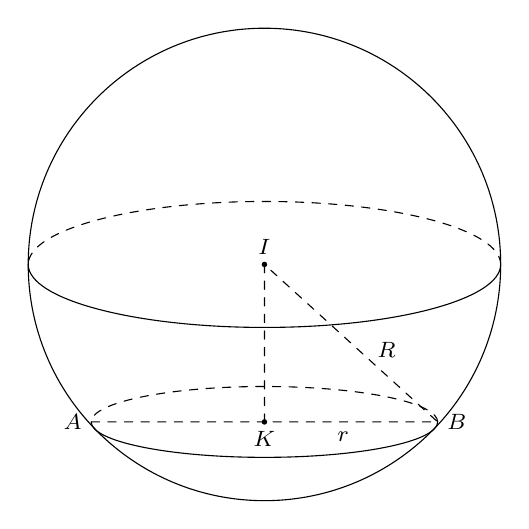
\begin{tikzpicture}[scale=1, font=\footnotesize, line join=round, line cap=round, >=stealth]
				\draw (0,0) circle (3);
				\draw[dashed] (3,0) arc [start angle=0,end angle=180,x radius=3,y radius=0.8];
				\draw (-3,0) arc [start angle=180,end angle=360,x radius=3,y radius=0.8];
				
				\draw[dashed] (2.2,-2) arc [start angle=0,end angle=180,x radius=2.2,y radius=0.45];
				\draw (-2.2,-2) arc [start angle=180,end angle=360,x radius=2.2,y radius=0.45];
				
				\draw (2.2,-2) node [right] {\footnotesize $B$};
				\draw (-2.2,-2) node [left] {\footnotesize $A$};
				\draw (0,0) node [above] {\footnotesize $I$};\fill (0,0) circle (1pt);
				\draw (1.55,-1.3) node [above] {\footnotesize $R$};
				\draw (1,-2) node [below] {\footnotesize $r$};
				\draw[dashed] (-2.2,-2)--(0,-2) (0,0)--(0,-2)--(2.2,-2)--(0,0);
				%Vẽ góc vuông
				\draw (0,-2) node [below] {\footnotesize $K$};\fill (0,-2) circle (1pt);
			\end{tikzpicture}
			
		\end{center}
		\begin{itemize}
			\item Mặt cầu $(S)$ có tâm $I(3 ;-2 ; 1) ; $ $R=10$.
			\item Khoảng cách từ $I$ đến $(P)$ là $I K=\mathrm{d} (I ;(P))=\dfrac{|6+4-1+9|}{3}=6$.
			\item Đường thẳng qua $I(3 ;-2 ; 1)$ vuông góc với $(P)$ có PTTS là $\heva{&x=3+2 t \\& y=-2-2 t \\& z=1-t.}$\\
			Khi đó, tọa độ tâm $K$ là nghiệm của hệ phương trình
			$$\heva{&x=3+2 t \\& y=-2-2 t \\& z=1-t \\& 2 x-2 y-z+9=0} \Rightarrow K(-1 ; 2 ; 3).$$
			\item  Bán kính $r=\sqrt{R^{2}-I K^{2}}=\sqrt{100-36}=8$.
		\end{itemize}
}\end{ex}

\begin{ex}%[2H5V3-4]
	Trong KG $Oxyz$, cho mặt phẳng $(P)\colon x-2y+2z-3=0$ và mặt cầu $(S)$ tâm $I(5;-3; 5)$, bán kính $R=2\sqrt{5}$. Từ một điểm $A$ thuộc mặt phẳng $(P)$ kẻ một đường thẳng tiếp xúc với mặt cầu $(S)$ tại $B$. Tính $OA$ biết $AB=4$.
	\choice
	{\True $OA=\sqrt{11}$}
	{$OA=5$}
	{$OA=3$}
	{$OA=\sqrt{6}$}
	\loigiai{
		Khoảng cách từ điểm $I$ đến mặt phẳng $(P)$ là $\mathrm{d}(I;(P))=\dfrac{|5-2\cdot(-3)+2\cdot 5-3|}{\sqrt{1^2+(-2)^2+2^2}}=6$.\\
		Ta có $AB$ tiếp xúc với $(S)$ tại $B$ nên tam giác $AIB$ vuông tại $B$, do đó ta có\\
		$IA=\sqrt{IB^2+AB^2}=\sqrt{R^2+AB^2}=\sqrt{(2\sqrt{5})^2+4^2}=6=d(I;(P)) \Rightarrow A$ là hình chiếu của $I$ lên $(P)$.\\
		Đường thẳng $IA$ đi qua điểm $I(5;-3; 5)$ có véc-tơ chỉ phương $\vec{u}=\overrightarrow{n}_(P)=(1;-2; 2)$ có phương trình $\heva{&x=5+t \\&y=-3-2t \\&z=5+2t.}$\\
		Ta có $A=IA\cap(P) \Rightarrow 5+t-2(-3-2t)+2(5+2t)-3=0\Rightarrow t=-2\Rightarrow A(3; 1; 1) \Rightarrow OA=\sqrt{11}$.}
\end{ex}

\begin{ex}%[2H5V3-4]
	Trong KG $Oxyz$, cho mặt cầu $(S)\colon x^2+y^2+z^2=9$ và điểm $M\left(x_0; y_0; z_0\right)$ thuộc $d\colon \heva{&x=1+t \\&y=1+2t \\&z=2-3t}$. Ba điểm $A$, $B$, $C$ phân biệt cùng thuộc mặt cầu sao cho $MA$, $MB$, $MC$ là tiếp tuyến của mặt cầu. Biết rằng mặt phẳng $(ABC)$ đi qua điểm $D(1; 1; 2)$. Tổng $T=x_0^2+y_0^2+z_0^2$ bằng
	\choice
	{$30$}
	{\True $26$}
	{$20$}
	{$21$}
	\loigiai{
		Mặt cầu $(S)$ có tâm $O(0; 0; 0)$ và bán kính $R=3$. Gọi $M\left(1+t_0; 1+2t_0; 2-3t_0\right) \in d$.\\
		Giả sử $T(x; y; z) \in(S)$ là một tiếp điểm của tiếp tuyến $MT$ với mặt cầu $(S)$. Khi đó 
		$$
		\begin{aligned}
			&OT^2+MT^2=OM^2\\
			& \Leftrightarrow 9+\left[x-\left(1+t_0\right)\right]^2+\left[y-\left(1+2 t_0\right)\right]^2+\left(z-\left(2-3 t_0\right)\right)^2=\left(1+t_0\right)^2+\left(1+2 t_0\right)^2+\left(2-3 t_0\right)^2 \\
			& \Leftrightarrow\left(1+t_0\right) x+\left(1+2 t_0\right)+\left(2-3 t_0\right) z-9=0.
		\end{aligned}
		$$
		Suy ra phương trình mặt phẳng $(ABC)$ có dạng $\left(1+t_0\right) x+\left(1+2t_0\right) y+\left(2-3t_0\right) z-9=0$.
		Do $D(1; 1; 2) \in(ABC)$ nên $1+t_0+1+2t_0+2.(2-3t)-9=0\Leftrightarrow t_0=-1\Rightarrow M(0;-1; 5)$.\\
		Vậy $T=0^2+(-1)^2+5^2=26$.
	}
\end{ex}

\begin{ex}%[2H5V1-7] 
	Trong KG $Oxyz$ cho hai điểm $A(0 ; 0 ; 3)$, $B(-2 ; 0 ; 1)$ và mặt phẳng $(\alpha)\colon 2 x-y+2 z+8=0$. Hỏi có bao nhiêu điểm $C$ trên mặt phẳng $(\alpha)$ sao cho tam giác $ABC$ đều?
	\choice
	{$2$}
	{$1$}
	{\True $0$}
	{Vô số}
	\loigiai{
		Gọi $(P)$ mặt phẳng trung trực của $A B$, khi đó phương trình của $(P)$ là $x+z-1=0$.\\
		Ta có $\overrightarrow{n}_P=(1 ; 0 ; 1),$ $ \overrightarrow{n}_{\alpha}=(2 ;-1 ; 2)$ nên $\left[\overrightarrow{n}_P, \overrightarrow{n}_{\alpha}\right]=(1 ; 0 ;-1)$.\\
		Gọi $d$ là giao tuyến của mặt phẳng $(P)$ với mặt phẳng $(\alpha)$. Chọn $\overrightarrow{u}_d=(1 ; 0 ;-1)$
		và điểm $M(1 ; 10 ; 0) \in d$ nên PTTS của $d$ là $\heva{&x=1+t \\& y=10 \\& z=-t.}$\\
		Do tam giác $A B C$ đều nên $C A=C B$ hay $C$ thuộc mặt phẳng trung trực của $A B$, mà $C \in(\alpha)$ nên $C \in(P) \cap(\alpha)=d$ suy ra tọa độ $C$ có dạng $C(1+t ; 10 ;-t)$.\\
		Do $\triangle A B C$ đều nên $A C=A B$, thay tọa độ các điểm ta có
		\allowdisplaybreaks
		\begin{eqnarray*}
			&&\sqrt{(1+t-0)^2+(10-0)^2+(-t-3)^2}=\sqrt{(-2-0)^2+(0-0)^2+(1-3)^2} \\&\Leftrightarrow& t^2+4 t+51=0\left(^{*}\right)
		\end{eqnarray*}
		Do phương trình $\left(^{*}\right)$ vô nghiệm nên không tồn tại điểm $C$ thỏa mãn yêu cầu bài toán.
		
}\end{ex}

\begin{ex}%[2H5V3-4] 
	Trong KG $Oxyz$, cho mặt cầu $(S)$ tâm $I(1 ; 3 ; 9)$ bán kính bằng $3$. Gọi $M$, $ N$ là hai điểm lần lượt thuộc hai trục $Ox$, $Oz$ sao cho đường thẳng $M N$ tiếp xúc với $(S)$, đồng thời mặt cầu ngoại tiếp tứ diện $OIMN$ có bán kính bằng $\dfrac{13}{2}$. Gọi $A$ là tiếp điểm của $M N$ và $(S)$, giá trị $A M \cdot A N$ bằng
	\choice
	{$39$}
	{\True $12 \sqrt{3}$}
	{$18$}
	{$28 \sqrt{3}$}
	\loigiai{
		\begin{itemize}
			\item Đặt $M(a ; 0 ; 0)$ và $N(0 ; 0 ; b)$. \\Nhận xét: $(S)$ tiếp xúc $(O x z)$ mà $M N \subset(O x z)$ tiếp xúc $(S)$ nên $M N$ tiếp xúc $(S)$ tại tiếp điểm của $(S)$ và $(O x z) \Rightarrow A(1 ; 0 ; 9)$.
			\item $\heva{&\overrightarrow{A M}=(a-1 ; 0 ;-9) \\& \overrightarrow{A N}=(-1 ; 0 ; b-9)} \Rightarrow \dfrac{a-1}{-1}=\dfrac{-9}{b-9} \Rightarrow(a-1)(b-9)=9$.
			\item Khi đó $O I M N$ có $\triangle O M N$ vuông tại $O,$ $(I M N) \perp(O M N)$ (do $I A \subset(I M N),$ $ I A \perp(O M N)$), suy ra bán kính mặt cầu ngoại tiếp $O I M N$ bằng bán kính đường tròn ngoại tiếp $\triangle I M N$ bằng $\dfrac{13}{2}$.\\
			Suy ra $\dfrac{1}{2} \cdot 3 \cdot M N=\dfrac{I M \cdot I N \cdot M N}{4 \cdot \dfrac{13}{2}} \Leftrightarrow I M \cdot I N=39$.\hfill(1)\\
			Mà 
			\allowdisplaybreaks
			\begin{eqnarray*}
				I M&=&\sqrt{(a-1)^2+3^2+9^2}=\sqrt{(a-1)^2+90}.\\
				I N&=&\sqrt{1^2+3^2+(b-9)^2}=\sqrt{10+\dfrac{81}{(a-1)^2}}.
			\end{eqnarray*}
			Thay vào (1) ta được
			$$\left[(a-1)^2+90\right]\left[10+\dfrac{81}{(a-1)^2}\right]=1521 \Leftrightarrow(a-1)^2=27.$$
			Ta có $\heva{&A M=\sqrt{(a-1)^2+81}=\sqrt{108}=6 \sqrt{3} \\& A N=\sqrt{1+(b-9)^2}=\sqrt{1+3}=2} \Rightarrow A M \cdot A N=12 \sqrt{3}$.
			
		\end{itemize}
}\end{ex}
\begin{ex}%[2H5V3-4] 
	Trong không gian $O x y z$, cho mặt cầu $(S)$ tâm $I(4 ; 1 ; 2)$ bán kính bằng $2$. Gọi $M$; $N$ là hai điểm lần lượt thuộc hai trục $O x$; $O y$ sao cho đường thẳng $M N$ tiếp xúc với $(S)$, đồng thời mặt cầu ngoại tiếp tứ diện $O I M N$ có bán kính bằng $\dfrac{7}{2}$. Gọi $A$ là tiếp điểm của $M N$ và $(S)$, giá trị $A M \cdot A N$ bằng
	\choice
	{\True $6 \sqrt{2}$}
	{$14$}
	{$8$}
	{$9 \sqrt{2}$}
	\loigiai{
		\begin{itemize}
			\item \textbf{Cách 1:}\\
			Ta có $\mathrm{d} (I,(O x y))=2$ nên mặt cầu $(S)$ tiếp xúc với mặt phẳng $(O x y)$ tại điểm $A(4 ; 1 ; 0)$, đồng thời đường thẳng $M N$ tiếp xúc với $(S)$ cũng tại điểm $A(4 ; 1 ; 0)$ do $M N \subset(O x y)$.\\
			Gọi $M(m ; 0 ; 0) ;$ $ N(0 ; n ; 0),$ $ m,$ $ n>0$.\\
			Do $A \in M N$ nên 
			\allowdisplaybreaks
			\begin{eqnarray*}
				{A M}=k \overrightarrow{A N} &\Rightarrow&\heva{&m-4=-4 k \\& -1=k(n-1)} \Rightarrow(m-4)(n-1)=4 \\&\Leftrightarrow& m=\dfrac{4 n}{n-1}, n-1 \neq 0.
			\end{eqnarray*}
			Phương trình mặt phẳng trung trực đoạn $O I\colon 4 x+y+2 z-\dfrac{21}{2}=0$.\\
			Phương trình mặt phẳng trung trực đoạn $O M\colon  x=\dfrac{m}{2}$.\\
			Phương trình mặt phẳng trung trực đoạn $O N\colon  y=\dfrac{n}{2}$.\\
			Do đó tâm mặt cầu ngoại tiếp tứ diện $O I M N$ là $J\left(\dfrac{m}{2} ; \dfrac{n}{2} ; \dfrac{-n^{2}+6 n-21}{4 n-4}\right)$.\\
			Theo giả thuyết cầu ngoại tiếp tứ diện $O I M N$ có bán kính bằng $\dfrac{7}{2}$ nên $O J=\dfrac{7}{2}$
			\allowdisplaybreaks
			\begin{eqnarray*}
				&\Leftrightarrow& O J^2=\dfrac{49}{4}\\&\Leftrightarrow& \dfrac{4 n^2}{(n-1)^2}+\dfrac{n^2}{4}+\dfrac{\left(n^2-6 n+21\right)^2}{16(n-1)^2}=\dfrac{49}{4}\\&\Leftrightarrow& n^{4}-4 n^{3}-10 n^2+28 n+49=0\\&\Leftrightarrow& n=1 \pm 2 \sqrt{2}.
			\end{eqnarray*}
			Vì $n>0$ nên chọn $n=1+2 \sqrt{2}$, suy ra $m=4+\sqrt{2}$.\\
			Khi đó $A M \cdot A N=6 \sqrt{2}$.
			\item \textbf{Cách 2:}\\
			Dễ thấy mặt cầu $(S)$ tiếp xúc với mặt phẳng $(O x y)$ tại điểm $A(4 ; 1 ; 0)$, đồng thời đường thẳng $M N$ tiếp xúc với $(S)$ cũng tại điểm $A(1 ; 4 ; 0)$ do $M N \subset(O x y)$.\\
			Gọi $M(a ; 0 ; 0) ; $ $N(0 ; b ; 0)$.\\
			Do $A \in M N$ nên $\overrightarrow{A M}=k \overrightarrow{A N} \Rightarrow\heva{&a-4=-4 k \\& -1=k(b-1)} \Rightarrow \dfrac{1}{b}+\dfrac{4}{a}=1$.\\
			Gọi $J$ là trung điểm $M N \Rightarrow J\left(\dfrac{a}{2} ; \dfrac{b}{2} ; 0\right)$ và $I(4 ; 1 ; 2)$ thuộc đường thẳng $\Delta$ vuông góc với $(O x y)$ tại điểm $J$. Phương trình $\Delta$ là $\heva{&x=\dfrac{a}{2} \\& y=\dfrac{b}{2} \\& z=t.}$\\
			Suy ra tâm của mặt cầu ngoại tiếp tứ diện $OIMN$ là điểm $K\left(\dfrac{a}{2} ; \dfrac{b}{2} ; t\right)$.\\
			Theo giả thiết ta có hệ 
			\allowdisplaybreaks
			\begin{eqnarray*}
				&&\heva{&\dfrac{1}{b}+\dfrac{4}{a}=1 \\& O K=\dfrac{7}{2} \\& I K=\dfrac{7}{2}} \Leftrightarrow \heva{&\dfrac{1}{b}+\dfrac{4}{a}=1 \\& \dfrac{a^2}{4}+\dfrac{b^2}{4}+t^2=\dfrac{49}{4} \\& \left(\dfrac{a}{2}-4\right)^2+\left(\dfrac{b}{2}-1\right)^2+(t-2)^2=\dfrac{49}{4}}\\&\Leftrightarrow&\heva{&a=\dfrac{4 b}{b-1} \\& 4 a+b+4 t-21=0 \\& \dfrac{a^2}{4}+\dfrac{b^2}{4}+t^2=\dfrac{49}{4}} \Leftrightarrow\heva{&a=\dfrac{4 b}{b-1} \\& t=\dfrac{b^2-6 b+21}{4(b-1)} \\& \dfrac{a^2}{4}+\dfrac{b^2}{4}+t^2=\dfrac{49}{4}}
				\\&\Rightarrow& \dfrac{b^2}{4}+\dfrac{4 b^2}{(b-1)^2}+\dfrac{\left(b^2-6 b+21\right)^2}{16(b-1)^2}=\dfrac{49}{4} \\&\Leftrightarrow& 4 b^2+64\left(1+\dfrac{1}{b-1}\right)^2+\left(b-5+\dfrac{16}{b-1}\right)^2=196
				\\&\Leftrightarrow& 4 b^2+64+\dfrac{128}{b-1}+\dfrac{64}{(b-1)^2}+(b-5)^2+32(b-5) \cdot \dfrac{1}{b-1}+\dfrac{256}{(b-1)^2}=196
				\\&\Leftrightarrow& 5 b^2-10 b+25+\dfrac{320}{(b-1)^2}+32(b-5+4) \cdot \dfrac{1}{b-1}=132 \\&\Leftrightarrow&(b-1)^2+\dfrac{64}{(b-1)^2}=16
				\Leftrightarrow\left[(b-1)^2-8\right]^2=0 \Leftrightarrow(b-1)^2=8 \\&\Leftrightarrow&\hoac{&b=1-2 \sqrt{2} \\& b=1+2 \sqrt{2}.}
			\end{eqnarray*}
			\begin{itemize}
				\item Với $b=1-2 \sqrt{2}$ ta được $a=4-\sqrt{2} \Rightarrow A M \cdot A N=6 \sqrt{2}$.
				\item Với $b=1+2 \sqrt{2}$ ta được $a=4+\sqrt{2} \Rightarrow A M \cdot  A N=6 \sqrt{2}$.
			\end{itemize}
		\end{itemize}
}\end{ex}

\Closesolutionfile{ans}
\indapan{10}{ans/ans-C5B3CD4_1-10-D3-LC}
\Opensolutionfile{ans}[ans/C5B3CD4_22-31-kq]
\TNSA
\begin{ex}%[2H5V3-4] 
	Trong không gian với hệ trục $Oxyz$, cho mặt cầu $(S)\colon  x^2+y^2+z^2-2 x-4 y+6 z-13=0$ và đường thẳng $d\colon  \dfrac{x+1}{1}=\dfrac{y+2}{1}=\dfrac{z-1}{1}$. Điểm $M(a ; b ; c),$ $(a>0)$ nằm trên đường thẳng $d$ sao cho từ $M$ kẻ được ba tiếp tuyến $M A, $ $M B,$ $ M C$ đến mặt cầu $(S)$ $(A,$ $ B,$ $ C$ là các tiếp điểm) và $\widehat{A M B}=60^{\circ},$ $ \widehat{BMC}=60^{\circ},$ $ \widehat{CMA}=120^{\circ}$. Biết $a^3+b^3+c^3=\dfrac{m}{n}$, tính $m+n$.
	\shortans[]{$121$}
	\loigiai{
		\begin{center}
			\begin{tikzpicture}[scale=1]
				\coordinate [label=left:$I$](I) at (0,0);
				\pgfmathsetmacro\a{sqrt(2.75)}
				\coordinate [label=above right:$A$](A) at (2.5,\a);
				\coordinate [label=below right:$C$](C) at (2.5,-\a);
				\coordinate (I') at ($(A)!1!90:(I)$);
				\draw (0,0) circle (3);
				\coordinate (J) at 
				(5,0);
				%gIAO ĐIỂM M
				\draw[name path=done,color=white] (I)--(J);
				\draw[name path=dtwo,color=white] (A)--(I');
				\path [name intersections={of=done and dtwo,by=M}];
				\draw (M) node[below right]{$M$};
				%gIAO ĐIỂM H
				\draw[name path=a] (I)--(M);
				\draw[name path=b] (A)--(C);
				\path [name intersections={of=a and b,by=H}];
				\draw (H) node[below left]{$H$};
				\foreach \diem in {A,I,C,M,H}	\fill (\diem)circle(1.5pt);		
				\draw[smooth](I)--(A)--(M)--(C)--(I);
				%	\draw[dashed](B)--(D);
			\end{tikzpicture}
		\end{center}
		Mặt cầu $(S)$ có tâm $I(1 ; 2 ;-3)$ và bán kính $R=\sqrt{1^2+2^2+(-3)^2+13}=3 \sqrt{3}$.\\
		Gọi $(C)$ là đường tròn giao tuyến của mặt phẳng $(A B C)$ và mặt cầu $(S)$.\\
		Đặt $M A=M B=M C=x$ khi đó $A B=x ;$ $ B C=x \sqrt{2} ; $ $C A=x \sqrt{3}$ do đó tam giác $A B C$ vuông tại $B$ nên trung điểm $H$ của $A C$ là tâm đường tròn $(C)$ và $H,$ $ I,$ $ M$ thẳng hàng.\\
		Vì $\widehat{AMC}=120^{\circ}$ nên tam giác $A I C$ đều do đó $x \sqrt{3}=R \Leftrightarrow x=3$ suy ra $I M=2 A M=2 x=6$.\\
		Lại có $M \in d$ nên $M(-1+t ;-2+t ; 1+t),$ $(t>1)$ mà $I M=6$ nên 
		\allowdisplaybreaks
		\begin{eqnarray*}
			(t-2)^2+(t-4)^2+(t+4)^2=36\Leftrightarrow 3 t^2-4 t=0 \Leftrightarrow \hoac{&t=0 \\& t=\dfrac{4}{3}.}
		\end{eqnarray*}
		Mà $a>0$ nên $t=\dfrac{4}{3}$ suy ra $H\left(\dfrac{1}{3} ;-\dfrac{2}{3} ; \dfrac{7}{3}\right)$. Vậy $a^3+b^3+c^3=\dfrac{112}{9}=\dfrac{m}{n}$.\\
		Khi đó $m+n=121$.
}\end{ex}

\begin{ex}%[2H5V3-4] 
	Trong không gian $O x y z$, cho mặt cầu $(S)$ tâm $I(1 ; 4 ; 2)$, bán kính bằng $2$. Gọi $M,$ $ N$ là hai điểm lần lượt thuộc hai trục $O x$, $ O y$ sao cho đường thẳng $M N$ tiếp xúc với $(S)$, đồng thời mặt cầu ngoại tiếp tứ diện $O I M N$ có bán kính bằng $\dfrac{7}{2}$. Gọi $A$ là tiếp điểm của $M N$ và $(S)$, tính giá trị $A M \cdot A N$ (làm tròn đến hàng phần trăm).
	\shortans[]{$8{,}48$}
	\loigiai{
		\begin{center}
			\begin{tikzpicture}[scale=1, line join=round, line cap=round, >=stealth]
				\coordinate [label=below:$O$](O) at (0,0);
				\coordinate [label=above right:$M$](M) at (5,0);
				\coordinate [label=below:$N$](N) at (-3,-2);
				\coordinate [label=above:$I$](I) at (2,4);
				\coordinate [label=below:$A$](A) at ($(N)! .75 ! (M)$);
				%gIAO ĐIỂM P
				\draw[name path=done] (I)--(N);
				\draw[name path=dtwo,color=white] (O)--($(O)! 1.5 ! (0,3)$);
				\path [name intersections={of=done and dtwo,by=P}];
				\draw[->] (M)--($(O)! 1.5 ! (M)$) node[below]{$x$};	
				\draw[->] (P)--($(O)! 3 ! (P)$) node[right]{$z$};	
				\draw[->] (N)--($(O)! 1.5 ! (N)$) node[below right]{$y$};	
				\foreach \diem in {O,M,N,I,A}	\fill (\diem)circle(1.5pt);	
				\draw[smooth](N)--(M)--(I) (A)--(I);
				\draw[dashed](P)--(O)--(M) (I)--(O)--(N);
			\end{tikzpicture}
		\end{center}
		Gọi $M(a ; 0 ; 0) \in O x,$ $ N(0 ; b ; 0) \in O y$.\\
		Ta có $\mathrm{d} (I ;(O x y))=2=R$ nên $(S)$ tiếp xúc với mặt phẳng $(O x y)$ tại điểm $A(1 ; 4 ; 0)$ và $M N$ cũng đi qua $A$.\\
		Lại có $\overrightarrow{A M}=(a-1 ;-4 ; 0), $ $\overrightarrow{A N}=(-1 ; b-4 ; 0)$ và $3$ điểm $A,$ $ M, $ $N$ thẳng hàng nên ta được $\dfrac{a-1}{-1}=\dfrac{-4}{b-4} \Leftrightarrow(a-1)(b-4)=4$.\\
		Tứ diện $O I M N$ có $I A \perp(O M N)$ và $\triangle O M N$ vuông tại $O$ nên nếu gọi $J$ là tâm mặt cầu ngoại tiếp tứ diện $O I M N$ thì $J \in(I M N)$.\\
		Suy ra bán kính mặt cầu ngoại tiếp tứ diện $OIMN$ bằng bán kính đường tròn ngoại tiếp $\triangle I M N$.\\
		Ta có $S_{\triangle I M N}=\dfrac{I M \cdot I N \cdot M N}{4 r}$ (với $r=\dfrac{7}{2}$ bán kính đường tròn ngoại tiếp $\triangle I M N$ ).
		\allowdisplaybreaks
		\begin{eqnarray*}
			&\Leftrightarrow& \dfrac{1}{2} I A \cdot M N=\dfrac{IM \cdot IN \cdot MN}{4 \cdot \dfrac{7}{2}} \Leftrightarrow I M \cdot I N=7\cdot IA \\&\Leftrightarrow& I M \cdot I N=14\Leftrightarrow\left[(a-1)^2+20\right]\left[(b-4)^2+5\right]=196. \quad(2)
		\end{eqnarray*}
		Đặt $\heva{&m=a-1 \\& n=b-4.}$
		Từ $(1)$ và $(2)$ ta có hệ $$\heva{&m n=4 \\& \left(m^2+20\right)\left(n^2+5\right)=196} \Leftrightarrow\heva{&n=\dfrac{4}{m}&(3) \\& \left(m^2+20\right)\left(\dfrac{16}{m^2}+5\right)=196&(4).}$$
		Từ $(4)$ ta được 
		\allowdisplaybreaks
		\begin{eqnarray*}
			&&\left(m^2+20\right)\left(16+5 m^2\right)=196 m^2\\
			&\Leftrightarrow& 5 m^4-80 m^2+320=0\\
			&\Leftrightarrow& m^2=8 \Leftrightarrow\hoac{&m=2 \sqrt{2} \\& m=-2 \sqrt{2}} \Rightarrow\hoac{&n=\sqrt{2} \\& n=-\sqrt{2}.}
		\end{eqnarray*}
		Suy ra $\hoac{&a=1+2 \sqrt{2},\, b=4+\sqrt{2} \\& a=1-2 \sqrt{2},\, b=4-\sqrt{2}.}$
		Vậy $A M \cdot A N=6 \sqrt{2}\approx 8{,}48$.
		
}\end{ex}

\begin{ex}%[2H5V3-4]
	Trong KG $Oxyz$ cho mặt cầu $(S)$ tâm $I(9; 3; 1)$ bán kính bằng $3$. Gọi $M, N$ là hai điểm lần lượt thuộc $2$ trục $Ox, Oz$ sao cho đường thẳng $MN$ tiếp xúc với $(S)$, đồng thời mặt cầu ngoại tiếp tứ diện $OIMN$ có bán kính bằng $\dfrac{13}{2}$. Gọi $A$ là tiếp điểm của $MN$ và $(S)$. Tính giá trị $AM\cdot AN$ (làm tròn đến hàng phần chục).
	\shortans[]{$20{,}8$}
	\loigiai{
		Ta có $\mathrm{d}(I;(Oxz))=3=R\Rightarrow(S)$ tiếp xúc với $(Oxz)$.\\
		Gọi $M(a; 0; 0) \in Ox$, $N(0; 0; b) \in Oz$.\\
		Ta có $MN$ tiếp xúc với $(S)$ tại $A$ nên $A$ là hình chiếu của $I$ lên $(Oxz)$.Suy ra $A(9; 0; 1)$.\\
		Gọi $K$ là trung điểm $MN\Rightarrow K\left(\dfrac{a}{2}; 0; \dfrac{b}{2}\right)$.\\
		Gọi $H$ là tâm mặt cầu ngoại tiếp tứ diện $OIMN\Rightarrow OH=\dfrac{13}{2} \Rightarrow HK\perp MN$.\\
		Gọi $T$ là trung điểm $\left.OM\Rightarrow \begin{array}{c}OM\perp KT\\ OM\perp HT\end{array}\right\} \Rightarrow OM\perp(KHT) \Rightarrow OM\perp HK\Rightarrow HK\perp(OMN)$.\\
		Mà $IA\perp(OMN) \Rightarrow HK\parallel IA$.\\
		Ta có $\overrightarrow{AI}=(0; 3; 0)$, $\overrightarrow{KH}=\left(x_H-\dfrac{a}{2}; y_H-0; z_H-\dfrac{b}{2}\right)$.\\
		$\overrightarrow{AI}$ cùng phương $\overrightarrow{KH}$ nên 
		$\heva{&x_H=\dfrac{a}{2} \\&y_H=c ~(c \neq 0) \\&z_H=\dfrac{b}{2}}$
		$\Rightarrow H\left(\dfrac{a}{2}; c; \dfrac{b}{2}\right)$.\\
		$OH=\dfrac{13}{2} \Rightarrow \dfrac{a^2}{4}+c^2+\dfrac{b^2}{4}=\dfrac{169}{4}$ \quad $(1)$. \\
		$HI=OH=\dfrac{13}{2} \Rightarrow\left(\dfrac{a}{2}-9\right)^2+(c-3)^2+\left(\dfrac{b}{2}-1\right)^2=\dfrac{169}{4}$ \quad $(2)$.\\
		Từ $(1)$ và $(2)$ suy ra $\dfrac{a^2}{4}+c^2+\dfrac{b^2}{4}=\left(\dfrac{a}{2}-9\right)^2+(c-3)^2+\left(\dfrac{b}{2}-1\right)^2$ \\
		$\Rightarrow 9a+b+6c=91$ \quad (3).\\
		$\overrightarrow{AM}=(a-9; 0;-1)$,
		$\overrightarrow{AN}=(-9; 0; b-1)$.\\
		Mặt khác $A, M, N$ thẳng hàng 
		\begin{eqnarray*}& \Rightarrow& \dfrac{a-9}{-9}=\dfrac{-1}{b-1}\\
			&\Leftrightarrow&(a-2)(b-1)=9 \\
			& \Leftrightarrow& a b-a-9b+9=9 \\
			& \Leftrightarrow& a b-a-9b=0\\
			& \Leftrightarrow& a(b-1)=a b\\
			& \Leftrightarrow& a=\dfrac{9b}{b-1}.
		\end{eqnarray*}
		Từ $(3) \Rightarrow 9\cdot \dfrac{9b}{b-1}+b+6c=91 \Leftrightarrow \dfrac{81b}{b-1}+b+6c=91$\\
		$\Leftrightarrow \dfrac{b^2+80b}{b-1}+6c=91\Leftrightarrow 6c=91-\dfrac{b^2+80b}{b-1}=\dfrac{-b^2+11b-91}{b-1}$\\
		$\Leftrightarrow c=\dfrac{-b^2+11b-91}{6(b-1)}$.\\
		Ta có $a^2+4c^2+b^2=169$\\
		$\Leftrightarrow\left(\dfrac{9b}{b-1}\right)^2+4\left(\dfrac{-b^2+11b-91}{6(b-1)}\right)^2+b^2=169$\\
		$\Leftrightarrow 9.81b^2+\left(b^4+121b^2+8281-22b^3+182b^2-2002b\right)+9b^2(b-1)^2=169.9.(b-1)^2$\\
		$\Leftrightarrow 729b^2+b^4+121b^2+8281-22b^3+182b^2-2002b+9b^4-18b^3+9b^2=1521b^2-3042b+1521$\\
		$\Leftrightarrow 10b^4-40b^3-480b^2+1040b+6760=0$\\
		$\Leftrightarrow\left[\begin{array}{l}b=1+3\sqrt{3} \Rightarrow a=\dfrac{9(1+3\sqrt{3})}{3\sqrt{3}}=9+\sqrt{3} \\ b=1-3\sqrt{3} \Rightarrow a=\dfrac{9(1-3\sqrt{3})}{-3\sqrt{3}}=9-\sqrt{3}.\end{array}\right.$
		\begin{itemize}
			\item Trường hợp 1: $ a=9+\sqrt{3}; b=1+3\sqrt{3} \Rightarrow \overrightarrow{AM}=(\sqrt{3}; 0;-1) \Rightarrow AM=2$.
		\end{itemize}
		$\Rightarrow \overrightarrow{AN}=(-9; 0; 3\sqrt{3}) \Rightarrow AN=\sqrt{108}$.\\
		Vậy $AM\cdot AN=2\cdot \sqrt{108}=12\sqrt{3}$.
		\begin{itemize}
			\item Trường hợp 2: $a=9-\sqrt{3}; b=1-3\sqrt{3} \Rightarrow \overrightarrow{AM}=(-\sqrt{3}; 0;-1) \Rightarrow AM=2$.
		\end{itemize}
		$\Rightarrow \overrightarrow{AN}=(-9; 0;-3\sqrt{3}) Vậy \Rightarrow AN=\sqrt{108}$.\\
		$AM\cdot AN=2\cdot \sqrt{108}=12\sqrt{3}$.
	}
\end{ex}

\begin{ex}%[2H5V3-2]
	Trong KG $Oxyz$, cho phương trình mặt cầu $\left(S_m\right)\colon x^2+y^2+z^2+(m+2) x+2m y-2m z-m-3=0$. Biết rằng với mọi số thực $m$ thì $\left(S_m\right)$ luôn chứa một đường tròn cố định. Tính bán kính $r$ của đường tròn đó (làm tròn đến hàng phần trăm).
	\shortans[]{$1{,}89$}
	\loigiai{
		Mặt cầu $\left(S_m\right)$ có tâm $I\left(-\dfrac{m+2}{2};-m; m\right)$ và bán kính $R=\dfrac{\sqrt{9m^2+8m+16}}{2}$.\\
		Với $m_1, m_2$ tùy ý và khác nhau, ta được hai phương trình mặt cầu tương ứng\\
		$\heva{&x^2+y^2+z^2+\left(m_1+2\right) x+2m_1y-2m_1z-m_1-3=0 \quad (1)\\
			&x^2+y^2+z^2+\left(m_2+2\right) x+2m_2y-2m_2z-m_2-3=0 \quad (2).}$\\
		Lấy (1) trừ (2) theo vế, ta được\\
		$\left(m_1-m_2\right) x+2\left(m_1-m_2\right) y-2\left(m_1-m_2\right) z-\left(m_1-m_2\right)=0$\\
		$\Leftrightarrow\left(m_1-m_2\right) \cdot(x+2y-2z-1)=0$\\
		$\Leftrightarrow x+2y-2z-1=0 \quad (3)$.\\
		Dễ thấy (3) là phương trình tổng quát của mặt phẳng. Suy ra
		họ mặt cầu $\left(S_m\right)$ có giao tuyến là đường tròn nằm trên mặt phẳng $(P)$ cố định có phương trình $x+2y-2z-1=0$.\\
		Mặt khác, đặt $d=d[I,(P)]=\dfrac{\left|-\dfrac{m+2}{2}-2m-2m-1\right|}{\sqrt{1^2+2^2+(-2)^2}}=\dfrac{|-9m-4|}{6}$.\\
		$\Rightarrow r^2=R^2-d^2=\dfrac{9m^2+8m+16}{4}-\dfrac{(-9m-4)^2}{36}=\dfrac{32}{9} \forall m \in \mathbb{R}$.\\
		Vậy $r=\dfrac{4\sqrt{2}}{3}\approx 1{,}89$.
	}
\end{ex}

\begin{ex}%[2H5V3-4]
	Trong không gian với hệ trục tọa độ $Oxyz$, cho đường thẳng $\Delta\colon \heva{&x=3+t \\&y=-1-t, \\&z=-2+t},(t \in \mathbb{R})$, điểm $M(1; 2;-1)$ và mặt cầu $(S)\colon x^2+y^2+z^2-4x+10y+14z+64=0$. Gọi $\Delta '$ là đường thẳng đi qua $M$ cắt đường thẳng $\Delta$ tại $A$, cắt mặt cầu tại $B$ sao cho $\dfrac{AM}{AB}=\dfrac{1}{3}$ và điểm $B$ có hoành độ là số nguyên. Phương trình mặt phẳng trung trực đoạn $AB$ có dạng $2x +by+cz+d=0$. Khi đó $b+c+d$ bằng
	\shortans[]{$-51$}
	\loigiai{
		$\Delta '$ là đường thẳng đi qua $M$ cắt đường thẳng  $\Delta$ tại $A$ suy ra tọa độ $A(3+a;-1-a;-2+a)$.\\
		Ta có $\dfrac{AM}{AB}=\dfrac{1}{3} \Leftrightarrow 3\overrightarrow{AM}=\pm \overrightarrow{AB}$.
		\begin{itemize}
			\item \textbf{Trường hợp 1:}\\
			$3\overrightarrow{AM}=\overrightarrow{AB} \Leftrightarrow \heva{&3(-2-a)=x-3-a \\
				&3(3+a)=y+1+a \\
				&3(1-a)=z+2-a} \Leftrightarrow\heva{&x=-3-2a \\
				&y=8+2a \\
				&z=1-2a
			}$.\\ 
			Suy ra $B(-3-2a; 8+2a; 1-2a)$.\\
			Do $B\in(S)$ nên\\
			$(-3-2a)^2+(8+2a)^2+(1-2a)^2-4(-3-2a)+10(8+2a)+14(1-2a)+64=0$
			$\Leftrightarrow 12a^2+40a+244=0$, phương trình vô nghiệm.
			\item \textbf{Trường hợp 2:}\\
			$3\overrightarrow{AM}=-\overrightarrow{AB} \Leftrightarrow \heva{&3(-2-a)=-(x-3-a) \\
				&3(3+a)=-(y+1+a) \\
				&3(1-a)=-(z+2-a)} \Leftrightarrow\heva{&x=9+4a \\
				&y=-10-4a \\
				&z=-5+4a
			}$\\
			Suy ra $B(9+4a;-10-4a;-5+4a)$.\\
			Do $B\in(S)$ nên\\
			$(9+4a)^2+(-10-4a)^2+(-5+4a)^2-4(9+4a)+10(-10-4a)+14(-5+4a)+64=0$
			$\Leftrightarrow 48a^2+112a+64=0\Leftrightarrow \hoac{&a=-1\\&a=-\dfrac{4}{3}}$.\\
			Điểm $B$ có hoành độ là số nguyên nên $B(5;-6;-9); A(2; 0;-3)$.\\
			Mặt phẳng trung trực đoạn $AB$ đi qua trung điểm $I\left(\dfrac{7}{2};-3;-6\right)$ và có một véc-tơ pháp tuyến $\vec{n}=(-1; 2; 2)$ nên có phương trình\\ $$\left(x-\dfrac{7}{2}\right)-2(y+3)-2(z+6)=0\Leftrightarrow 2x-4y-4z-43=0.$$
			Khi đó $b+c+d=-51$.
		\end{itemize}
	}
\end{ex}

\begin{ex}%[2D1H3-6]
	Một doanh nghiệp dự kiến lợi nhuận khi sản xuất $x$ sản phẩm ($0\leq x\leq 300$) được cho bởi hàm số $y=-x^3 + 300x^2$ (đơn vị: đồng).
	\begin{enumerate}
		\item Nêu ra các khoảng số lượng sản phẩm mà doanh nghiệp luôn có lợi nhuận?
		\item Nêu ra các khoảng số lượng sản phẩm mà doanh nghiệp luôn thiệt hại?
		\item So sánh lợi nhuận khi sản xuất $100$ sản phẩm, $200$ sản phẩm và $300$ sản phẩm?
		\item Doanh nghiệp cần sản xuất bao nhiêu sản phẩm để đạt lợi nhuận lớn nhất? Lợi nhuận lớn nhất đó là bao nhiêu?
		\item Nếu doanh nghiệp muốn duy trì lợi nhuận không dưới $2.000.000$ đồng, họ nên sản xuất ít nhất bao nhiêu sản phẩm và không vượt quá bao nhiêu sản phẩm?
	\end{enumerate}
	\loigiaiEX{
		\begin{enumerate}
			\item Ta có $y'=-3x^2+600x$.\\
			Cho $y'=0\Leftrightarrow -3x^2+600x=0\Leftrightarrow x=0\vee x= 200$.
			\begin{center}
				
\begin{tikzpicture}[scale=1, font=\footnotesize, line join=round, line cap=round, >=stealth]
					\tkzTabInit[nocadre=false,lgt=1.2,espcl=3.2,deltacl=0.5]
					{$x$/.7 ,$y'$/.7,$y$/2}
					{$0$ , $200$ , $300$}
					\tkzTabLine{ , + , $0$ , - , }
					\tkzTabVar{-/$f(0)$, +/$f(200)$, -/$f(300)$}
				\end{tikzpicture}
			\end{center}
			Như vậy doanh nghiệp luôn có lợi nhuận khi số lượng sản phẩm sản xuất ra nằm trong khoảng $(0; 200)$.
			\item Như vậy doanh nghiệp luôn thiệt hại khi số lượng sản phẩm sản xuất ra nằm trong khoảng $(0; 200)$.
			\item Ta có
			\begin{itemize}
				\item Lợi nhuận khi sản xuất $100$ sản phẩm
				$y(100)= 2.000.000$ đồng.
				\item Lợi nhuận khi sản xuất $200$ sản phẩm
				$y(200)= 4.000.000$ đồng.
				\item Lợi nhuận khi sản xuất $300$ sản phẩm
				$y(300)= 0$ đồng.
			\end{itemize}
			Như vậy lợi nhuận khi sản xuất $200$ sản phẩm là lớn nhất. Lợi nhuận khi sản xuất $100$ sản phẩm lớn hơn lợi nhuận khi sản xuất $300$ sản phẩm.
			\item Lợi nhuận khi sản xuất $200$ sản phẩm là lớn nhất. Lợi nhuận lớn nhất đó bằng $4.000.000$ đồng.
			\item Để doanh nghiệp có lợi nhuận không dưới $2.000.000$ đồng, ta cần giải bất phương trình
			$y(x)\geq 2.000.000 \Leftrightarrow -x^3 + 300x^2 - 2.000.000 \geq 0 \Leftrightarrow x \leq -73{,}2 \vee 100\leq x \leq 273{,}2$.\\
			Như vậy để doanh nghiệp có lợi nhuận không dưới $2.000.000$ đồng thì họ nên sản xuất ít nhất $100$ sản phẩm và không vượt quá $273$ sản phẩm.
		\end{enumerate}
	}
\end{ex}

%%==============Cau_EX4==============%%%
\begin{ex}
	Trong KG $Oxyz$, cho phương trình mặt cầu $(S_m)\colon x^2+y^2+z^2+(m+2) x+2m y-2m z-m-3=0$. Biết rằng với mọi số thực $m$ thì $(S_m)$ luôn chứa một đường tròn cố định. Tính bán kính $r$ của đường tròn đó (làm tròn kết quả đến hàng phần mười).
	\shortans{$1{,}9$}
	\loigiai{
		Mặt cầu $(S_m)$ có tâm $I\left(-\dfrac{m+2}{2};-m; m\right)$ và bán kính $R=\dfrac{\sqrt{9m^2+8m+16}}{2}$.\\
		Với $m_1$, $m_2$ tùy ý và khác nhau, ta được hai phương trình mặt cầu tương ứng:
		$$\heva{&x^2+y^2+z^2+\left(m_1+2\right) x+2m_1 y-2m_1 z-m_1-3=0\\ &x^2+y^2+z^2+\left(m_2+2\right) x+2m_2 y-2m_2 z-m_2-3=0.}$$
		Lấy $(1)$ trừ $(2)$ theo vế, ta được
		\allowdisplaybreaks
		\begin{eqnarray*}
			&&\left(m_1-m_2\right) x+2\left(m_1-m_2\right) y-2\left(m_1-m_2\right) z-\left(m_1-m_2\right)=0
			\\
			&\Leftrightarrow&\left(m_1-m_2\right) \cdot(x+2y-2z-1)=0
			\\
			&\Leftrightarrow& x+2y-2z-1=0. \qquad(3)		
		\end{eqnarray*}
		Dễ thấy $(3)$ là phương trình tổng quát của mặt phẳng.\\
		Suy ra họ mặt cầu $(S_m)$ có giao tuyến là đường tròn nằm trên mặt phẳng $(P)\colon x+2y-2z-1=0$ cố định.\\
		Mặt khác, đặt $d=\mathrm{d}\left[I,(P)\right]=\dfrac{\left|-\dfrac{m+2}{2}-2m-2m-1\right|}{\sqrt{1^2+2^2+(-2)^2}}=\dfrac{|-9m-4|}{6}$.\\
		$\Rightarrow r^2=R^2-d^2=\dfrac{9m^2+8m+16}{4}-\dfrac{(-9m-4)^2}{36}=\dfrac{32}{9} \quad \forall m \in \mathbb{R}$.\\
		Vậy $r=\dfrac{4\sqrt{2}}{3}\approx 1{,}9$.
	}
\end{ex}
%%%==============HetCau_EX4==============%%%

%%%==============Cau_EX5==============%%%
\begin{ex}
	Trong không gian với hệ trục tọa độ $Oxyz$, cho đường thẳng $\Delta\colon \heva{&x=3+t \\ &y=-1-t, \\ &z=-2+t}(t \in \mathbb{R})$, điểm $M(1; 2;-1)$ và mặt cầu $(S)\colon x^2+y^2+z^2-4x+10y+14z+64=0$. Gọi $\Delta'$ là đường thẳng đi qua $M$ cắt
	đường thẳng $\Delta$ tại $A$, cắt mặt cầu tại $B$ sao cho $\dfrac{AM}{AB}=\dfrac{1}{3}$ và điểm $B$ có hoành độ là số nguyên. Biết  phương trình mặt phẳng trung trực đoạn $AB$ có dạng $ax+by+cz+d=0$. Tình $2a+b-12c+d$.
	\shortans{$5$}
	\loigiai{
		$\Delta'$ là đường thẳng đi qua $M$ cắt đường thẳng $\Delta$ tại $A$ suy ra tọa độ $A(3+a;-1-a;-2+a)$.\\
		$\dfrac{AM}{AB}=\dfrac{1}{3} \Leftrightarrow 3\overrightarrow{AM}=\pm \overrightarrow{AB}$.
		\begin{itemize}
			\item Trường hợp $1$:\\
			$3\overrightarrow{AM}=\overrightarrow{AB} \Leftrightarrow\heva{&3(-2-a)=x-3-a \\ &3(3+a)=y+1+a \\ &3(1-a)=z+2-a} \Leftrightarrow\heva{&x=-3-2a \\ &y=8+2a \\ &z=1-2a.}$\\
			Suy ra $B(-3-2a; 8+2a; 1-2a)$.\\
			Do $B\in(S)$ nên
			\allowdisplaybreaks
			\begin{eqnarray*}
				&&(-3-2a)^2+(8+2a)^2+(1-2a)^2-4(-3-2a)+10(8+2a)+14(1-2a)+64=0
				\\
				&\Leftrightarrow& 12a^2+40a+244=0,~\text{phương trình vô nghiệm}			
			\end{eqnarray*}
			\item Trường hợp $2$:\\
			$3\overrightarrow{AM}=-\overrightarrow{AB} \Leftrightarrow\heva{&3(-2-a)=-(x-3-a) \\& 3(3+a)=-(y+1+a) \\ &3(1-a)=-(z+2-a)} \Leftrightarrow\heva{&x=9+4a \\ &y=-10-4a \\ &z=-5+4a.}$\\
			Suy ra $B(9+4a;-10-4a;-5+4a)$.\\
			Do $B\in(S)$ nên
			\allowdisplaybreaks
			\begin{eqnarray*}
				&&(9+4a)^2+(-10-4a)^2+(-5+4a)^2-4(9+4a)+10(-10-4a)+14(-5+4a)+64=0
				\\
				&\Leftrightarrow& 48a^2+112a+64=0
				\\
				&\Leftrightarrow&\hoac{&a=-1\\ &a=-\dfrac{4}{3}.}			
			\end{eqnarray*}
			Điểm $B$ có hoành độ là số nguyên nên $B(5;-6;-9)$; $A(2; 0;-3)$.\\
			Mặt phẳng trung trực đoạn $AB$ đi qua trung điểm $I\left(\dfrac{7}{2};-3;-6\right)$ và có một véc-tơ pháp tuyến $\vec{n}=(-1; 2; 2)$ nên có phương trình \[\left(x-\dfrac{7}{2}\right)-2(y+3)-2(z+6)=0\Leftrightarrow 2x-4y-4z-43=0.\]
			Suy ra $a=2$, $b=-4$, $c=-4$, $d=-43$.
		\end{itemize}
		Vậy $2a+b-12c+d=2\cdot 2+(-4)-12\cdot (-4)+(-43)=5$.
	}
\end{ex}
%%%==============HetCau_EX5==============%%%

%%%==============Cau_EX6==============%%%
\begin{ex}
	Trong KG $Oxyz$, cho $(S)\colon (x+3)^2+(y-2)^2+(z-5)^2=36$, điểm $M(7;1;3)$. Gọi $\Delta$ là đường thẳng di động luôn đi qua $M$ và tiếp xúc với mặt cầu $(S)$ tại $N$. Tiếp điểm $N$ di động trên đường tròn $(T)$ có tâm $J(a;b;c)$. Gọi $k=2a-5b+10c$, tính giá trị của $k$.
	\shortans{$50$}
	\loigiai{
		\immini{	Mặt cầu $(S)\colon (x+3)^2+(y-2)^2+(z-5)^2=36$ có tâm $I(-3;2;5)$, bán kính $R=6$.\\
			Có $IM=\sqrt{25+16+4}=3\sqrt{5} > 6=R$, nên $M$ thuộc miền ngoài của mặt cầu $(S)$.\\
			Có $MN$ tiếp xúc mặt cầu $(S)$ tại $N$, nên $MN\perp IN$ tại $N$.\\
			Gọi $J$ là điểm chiếu của $N$ lên $MI$.\\
			Có $IN^2=IJ\cdot IM$. Suy ra $IJ=\dfrac{IN^2}{IM}=\dfrac{36}{3\sqrt{5}}=\dfrac{12\sqrt{5}}{5}$ (không đổi), $I$ cố định.\\
			Suy ra $N$ thuộc $(P)$ cố định và mặt cầu $(S)$, nên $N$ thuộc đường tròn $(C)$ tâm $J$.}{	\begin{tikzpicture}[scale=0.7]
				\tikzset{declare function={%
						R=3;d=-1.5;theta=65;
						r=sqrt(R*R-d*d);betacrit=asin(d/r*cot(theta));},samples=200,smooth}
				\tdplotsetmaincoords{theta}{0}
				\draw (0,0) coordinate (I) circle (R);
				\path (-90:R) coordinate (A);
				\begin{scope}[tdplot_main_coords,line join=round]
					\draw[dashed,dash pattern = on 2pt off 1.5pt]
					(I)--(0,0,d) coordinate (J)
					--({r*cos(betacrit)},{r*sin(betacrit)},d) coordinate (N) -- cycle
					(J)--(A)
					plot[variable=\t,domain=betacrit:180-betacrit]({r*cos(\t)},{r*sin(\t)},d)
					plot[variable=\t,domain=0:180]({R*cos(\t)},{R*sin(\t)},0);
					\draw plot[variable=\t,domain=betacrit:-180-betacrit]({r*cos(\t)},{r*sin(\t)},d);
					\draw plot[variable=\t,domain=180:360]({R*cos(\t)},{R*sin(\t)},0);
				\end{scope}
				\path ($(A)!-0.56!(I)$) coordinate (M);
				\draw (A)--(M)--(N);
				\foreach \t/\g in {I/90,N/-30,J/220,M/-90}{
					\draw[fill=black] (\t) circle (1pt) node[shift={(\g:7pt)},font=\scriptsize]{$ \t $};
				}
		\end{tikzpicture}}\noindent
		Gọi $N(x;y;z)$, có $\overrightarrow{IJ}=\dfrac{IJ}{IM}\cdot \overrightarrow{IM}=\dfrac{12\sqrt{5}}{5}\cdot \dfrac{1}{3\sqrt{5}} \overrightarrow{IM}=\dfrac{4}{5} \overrightarrow{IM} \Leftrightarrow\heva{&x+3=8\\ &y-2=-\dfrac{4}{5} \\ &z-5=-\dfrac{2}{5}.}$\\
		Suy ra $ N\left(5; \dfrac{6}{5}; \dfrac{23}{5}\right)$, $k=2a-5b+10c=50$. \\
		Vậy $k=50$.
	}
\end{ex}
%%%==============HetCau_EX6==============%%%

%%%==============Cau_EX7==============%%%
\begin{ex}
	Trong KG $Oxyz$, cho mặt cầu $(S)\colon x^2+y^2+z^2-4x+4y-2z-7=0$ và đường thẳng $d_m$ là giao tuyến của hai mặt phẳng $x+(1-2m) y+4m z-4=0$ và $2x+m y-(2m+1) z-8=0$. Khi đó $m$ thay đổi các giao điểm của $d_m$ và $(S)$ nằm trên một đường tròn cố định. Tính bán kính $r$ của đường tròn đó (làm tròn kết quả đến hàng phần mười).
	\shortans{$3{,}1$}
	\loigiai{
		%Hình vẽ
		Giả sử đường thẳng $d_m$ cắt mặt cầu tại hai điểm $A$, $B$.\\
		Mặt cầu $(S)$ có tâm $I(2;-2; 1)$, bán kính $R=4$.\\
		Đường thẳng $M(x; y) \in d_m$ thỏa $\heva{&x+(1-2m) y+4m z-4=0\\ &2x+m y-(2m+1) z-8=0} \Rightarrow 5x+y-2z-20=0$ nên các giao điểm của $(S)$ và $d_m$ thuộc đường tròn giao tuyến giữa $(S)$ và $(P)\colon 5x+y-2z-20=0$.\\
		$\mathrm{d}\left(I,(P)\right)=\dfrac{14}{\sqrt{30}}$ nên $r=\sqrt{R^2-\mathrm{d}^2(I,(P))}=\sqrt{4^2-\dfrac{14^2}{30}}=\sqrt{\dfrac{142}{15}}\approx 3{,}1$.
	}
\end{ex}
%%%==============HetCau_EX7==============%%%
\Closesolutionfile{ans}
\indapan{6}{ans/C5B3CD4_22-31-kq}